\documentclass[11pt]{article}
\usepackage[T1]{fontenc}
\usepackage{lmodern}
\usepackage[margin=1.05in]{geometry}
\usepackage{amsmath,amssymb,amsthm,mathtools}
\usepackage{microtype,enumitem,booktabs}
\usepackage{tikz}
\usetikzlibrary{arrows.meta,positioning}
\usepackage[colorlinks=true,linkcolor=blue!45!black,citecolor=blue!45!black,urlcolor=blue!45!black]{hyperref}
\usepackage[nameinlink,noabbrev]{cleveref}
\newtheorem{theorem}{Theorem}[section]
\newtheorem{lemma}[theorem]{Lemma}
\newtheorem{proposition}[theorem]{Proposition}
\newtheorem{corollary}[theorem]{Corollary}
\theoremstyle{definition}
\newtheorem{definition}[theorem]{Definition}
\theoremstyle{remark}
\newtheorem{remark}[theorem]{Remark}
\newcommand{\C}{\mathbb C}
\newcommand{\R}{\mathbb R}
\newcommand{\Z}{\mathbb Z}
\newcommand{\N}{\mathbb N}
\DeclareMathOperator{\HS}{HS}
\DeclareMathOperator{\HH}{HH}
\DeclareMathOperator{\tr}{tr}
\DeclareMathOperator{\supp}{supp}
\DeclareMathOperator{\con}{con}
\DeclareMathOperator{\id}{id}
\numberwithin{equation}{section}
\setlist{itemsep=3pt,topsep=5pt}
\setlength{\emergencystretch}{1.5em}
\pdfinfoomitdate=1
\pdftrailerid{}
\pdfsuppressptexinfo=15
\hypersetup{pdftitle={The Bass trace conjecture and the characteristic-zero Kaplansky idempotent conjecture},pdfauthor={OpenAI}}
\title{The Bass trace conjecture and the characteristic-zero Kaplansky idempotent conjecture}
\author{OpenAI}
\date{September 24, 2026}
\begin{document}
\maketitle
\begin{abstract}
We prove the complex group-ring Bass trace conjecture for every discrete
group: the Hattori--Stallings trace of a finitely generated projective module
over its complex group ring is supported on conjugacy classes of finite-order
elements. As a consequence, for every torsion-free group $G$ and every
commutative unital domain $R$ of characteristic zero, the only idempotents
in $RG$ are $0$ and $1$. This proves Kaplansky's idempotent conjecture in
characteristic zero.
\end{abstract}
\tableofcontents
\section{Introduction}
\label{sec:introduction}

The rank of a projective module over a group ring contains information
about individual conjugacy classes. This refinement of ordinary rank is
a basic ingredient of group-ring Euler characteristics: alternating sums
of projective-module ranks retain information that a numerical Euler
characteristic forgets \cite{Bass1976,Bass1979}. The Bass trace conjecture
asks how much of that information can occur at elements of infinite order.
We first specify the complex version of this question.

For a unital complex algebra $A$, let $K_0(A)$ be the Grothendieck group of
finitely generated projective right $A$-modules, and set
\[
 \HH_0(A)=A/[A,A],
\]
where $[A,A]$ is the complex linear span of commutators. An idempotent
$e=(e_{ij})\in M_q(A)$ represents the projective right module
$eA^q$, with matrices acting on columns by left multiplication. Its
Hattori--Stallings trace is
\[
 \HS_A([eA^q])=\left[\sum_{i=1}^q e_{ii}\right]\in\HH_0(A),
\]
extended additively to virtual projective classes.

Let $G$ be a discrete group and write $\con(G)$ for its set of conjugacy
classes. The quotient $\HH_0(\C G)$ identifies with
$\bigoplus_{C\in\con(G)}\C C$ by
\begin{equation}\label{eq:class-trace}
 \left[\sum_{h\in G}a_hh\right]
 \longmapsto
 \sum_{C\in\con(G)}\left(\sum_{h\in C}a_h\right)C.
\end{equation}
Indeed, a commutator has zero sum on each conjugacy class, and the
differences of conjugate group elements span the kernel of the displayed
map. Such differences are commutators: $tst^{-1}-s=[t,st^{-1}]$.
All sums arising from an element of $\C G$ have finite support.
We write $\HS_G(x)(C)$ for the coefficient at $C$.

The complex group-ring Bass conjecture asks whether these coefficients
vanish on every infinite-order conjugacy class, for every group and every
class in $K_0(\C G)$; see
\cite[Conjecture 2.1]{BCM2004} and \cite[Conjecture 2]{CM2011}.

\begin{theorem}\label{thm:bass}
Let $G$ be any discrete group. For every $x\in K_0(\C G)$ and every
infinite-order element $g\in G$,
\[
 \HS_G(x)([g]_G)=0.
\]
Equivalently, if $\con_{\mathrm{fin}}(G)$ denotes the conjugacy classes of
finite-order elements, then
\[
 \HS_G\bigl(K_0(\C G)\bigr)
 \subseteq\bigoplus_{C\in\con_{\mathrm{fin}}(G)}\C C.
\]
\end{theorem}

This resolves the complex group-ring formulation positively. Finite-order
coefficients need not vanish away from the identity: for a finite group
$F$, the idempotent $|F|^{-1}\sum_{h\in F}h$ has coefficient
$|C|/|F|$ at every conjugacy class $C$. The conclusion therefore differs
from the identity-only support assertion for integral group rings.
That integral assertion follows in Section~\ref{sec:completion} by combining
Theorem~\ref{thm:bass} with the known restriction on its finite-order
coefficients.

\subsection{Trace rank and the idempotent conjecture}

For a torsion-free group the identity is the only finite-order element,
so Theorem~\ref{thm:bass} also has numerical and ring-theoretic
consequences. Define the canonical trace and the augmentation by
\[
 \tau_G\!\left(\sum_{g\in G}a_g g\right)=a_1,\qquad
 \epsilon_G\!\left(\sum_{g\in G}a_g g\right)=\sum_{g\in G}a_g.
\]
For a matrix $b=(b_{ij})\in M_q(\C G)$, put
$\tau_{G,q}(b)=\sum_{i=1}^q\tau_G(b_{ii})$, and let
$\epsilon_{G,q}(b)\in M_q(\C)$ be the entrywise augmentation.
The coefficient at $[1]_G$ of the Hattori--Stallings trace defines
\[
 \tau_{G,*}:K_0(\C G)\longrightarrow\C,\qquad
 \tau_{G,*}([e(\C G)^q])=\tau_{G,q}(e).
\]
The augmentation also defines the integer-valued augmentation rank
\[
 \operatorname{rk}_{\epsilon}:K_0(\C G)
 \xrightarrow{(\epsilon_G)_*}K_0(\C)
 \xrightarrow{\dim_{\C}}\Z.
\]

The idempotent conjecture commonly attributed to Kaplansky asks whether,
for every torsion-free group $G$ and every field $k$, an element
$e\in kG$ satisfying $e^2=e$ must be $0$ or $1$; see
\cite[Problem 3]{OW2023}. It concerns elements of the group ring itself,
not arbitrary idempotent matrices over that ring.

\begin{corollary}\label{cor:torsion-free}
Let $G$ be any torsion-free discrete group.
\begin{enumerate}[label=\textup{(\roman*)}]
 \item For every $q\geq1$ and every idempotent $e\in M_q(\C G)$,
 \[
  \tau_{G,q}(e)=\operatorname{rank}_{\C}\bigl(\epsilon_{G,q}(e)\bigr).
 \]
 Consequently $\tau_{G,*}=\operatorname{rk}_{\epsilon}$, with
 $\Z$ viewed as a subgroup of $\C$, and
 \[
  \tau_{G,*}\bigl(K_0(\C G)\bigr)=\Z.
 \]
 \item For every commutative unital domain $R$ of characteristic zero,
 every $e\in RG$ satisfying $e^2=e$ is either $0$ or $1$.
\end{enumerate}
\end{corollary}

Part \textup{(ii)} resolves the characteristic-zero Kaplansky idempotent
conjecture positively, and includes coefficient domains as well as fields.
Section~\ref{sec:torsion-free} derives both parts from the trace theorem.
The integer range in part \textup{(i)} concerns algebraic $K_0(\C G)$;
its relation to the reduced $C^*$-completion is made explicit there.

The integral trace consequence also links the theorem to fixed-point
theory. A map $f$ is a \emph{homotopy idempotent} if $f\circ f\simeq f$.
Berrick, Chatterji and Mislin's equivalences \cite[Theorems 1--2]{BCM2006}
then imply that every homotopy idempotent on a connected closed smooth
oriented manifold of dimension greater than two is freely homotopic to
a map with exactly one fixed point. They also identify ordinary and
$L^2$-Lefschetz numbers for pointed homotopy idempotents of connected
closed smooth oriented manifolds that induce the identity on the
fundamental group.
Corollary~\ref{cor:homotopy-idempotents} states these consequences precisely;
Section~\ref{sec:completion} explains their connection to projective
Euler characteristics.

\subsection{The two parts of the proof}

We first describe the algebraic construction to explain the geometric
statement it needs. The body of the paper begins with that geometric
statement, formulated independently of group rings, and completes its
proof before constructing the cycles and cocycles to which it applies.

For a finitely generated group $G$, the algebraic construction starts
with an idempotent $e\in M_q(\C G)$ and one infinite-order element
$g\in G$. The finitely many nonzero group coefficients of $e$ determine
a finite set of steps. Products of matrix
coefficients along paths from $h$ to $gh$, followed by the ordinary
matrix trace, give complex weights on finite lists of group elements.
Idempotency says that summing over any intermediate vertex removes that
vertex. Cyclicity of matrix trace gives a second identity, a cyclic shift
whose last vertex is multiplied by $g$.

Project the vertices to the coset set $Y=\langle g\rangle\backslash G$.
The group $H=C_G(g)/\langle g\rangle$, where $C_G(g)$ is the centralizer
of $g$, acts freely on $Y$. For every positive even dimension $2m$, the weighted
lists define a simplicial cycle modulo this action. Its simplices use
connected sets of vertices in one graph of bounded degree, fixed as $m$
increases. A Pfaffian cocycle evaluates on this cycle as
$2^{-m}\HS_G([e(\C G)^q])([g]_G)$. Here a cocycle means an alternating
function on vertex lists that vanishes on simplicial boundaries. The
explicit construction and the evaluation occupy
Sections~\ref{sec:idempotents} and~\ref{sec:detector}.

The geometric part, proved first in Sections~\ref{sec:framework}--\ref{sec:chains},
shows that every invariant cocycle evaluates to zero on cycles of this
kind in sufficiently high dimension. We cut the supporting simplicial
complex successively into pieces of bounded diameter, choosing the
separating sets nearly to minimize their areas. A volume estimate and
repeated slicing make the expected number of points in the final
zero-dimensional set arbitrarily small. A subdivision construction turns
this point count into a bound for cocycle evaluations. Equivariant chain
homotopy keeps the evaluation unchanged throughout the construction.

The fixed graph degree makes increasing the dimension useful. Through
each vertex there are only exponentially many connected vertex sets of a
given size. On an $n$-simplex, Euclidean structures chosen from spanning
trees of its vertex set give volume $1/n!$; repeated slicing produces the
same factorial in the comparison with a point of the final separating
set. After these factors cancel, radii chosen in terms of the fixed
degree bound make the remaining volume ratio tend to zero with $n$.
The local replacement argument turns this strict volume margin into the
small expected point count. No homological-dimension bound on $H$ is
assumed.

Two features permit this argument for arbitrary groups. A compact
probability space with a free action separates overlapping translates of
local modifications, without any amenability assumption. Also, each top
simplex has its own averaged Euclidean area functional. The areas need
not match along common faces; the successive cuts keep the relevant
dimensional measures away from those faces.
The cocycles need not be globally bounded: near each original simplex,
the construction uses only a fixed finite set of possible vertices.
Bounding the cocycle on those lists suffices for the evaluation estimate.

The final assembly in Section~\ref{sec:completion} chooses a large even
dimension, forcing the individual trace coefficient to vanish. Passing
from finitely generated groups to arbitrary groups uses the exact sum
over subgroup conjugacy classes contained in an ambient conjugacy class.
Section~\ref{sec:torsion-free} then extracts the augmentation rank from
the identity coefficient. In the scalar case this rank is $0$ or $1$,
and the standard faithful-trace argument forces the idempotent itself
to be $0$ or $1$. A finite-coefficient reduction extends that conclusion
from complex coefficients to every commutative characteristic-zero domain.

\subsection{Relation to previous work}

The rank construction comes from Hattori and Stallings
\cite{Hattori1965,Stallings1965}; Bass developed its relation to Euler
characteristics and formulated the integral conjecture in
\cite{Bass1976}; see also \cite[Conjecture (4.5)]{Bass1979}.
Bass proved complex trace vanishing at infinite-order elements for linear
groups \cite[Theorem (6.1)(f)]{Bass1979}. For the integral trace,
Linnell established a restriction on the possible nonzero coefficients
\cite[Lemma 4.1]{Linnell1983}, later recovered through topological
Hochschild homology by Berrick and Hesselholt \cite[Theorem A]{BH2015}.
Its finite-order consequence is the input used in
Section~\ref{sec:completion}.

The scalar idempotent problem also has a long history of trace methods.
Formanek proved the characteristic-zero conclusion for torsion-free
groups satisfying the ascending chain condition on subgroups
\cite[Theorem 1]{Formanek1973}. Burger and Valette revisit the theorems of
Kaplansky and Zalesskii: the canonical trace of a complex scalar
idempotent lies in $[0,1]$, its endpoints force the idempotent to be
trivial, and its value is rational
\cite[Theorems 1.3 and 2.1]{BV1998}. They also obtain
$\tau_{G,*}(K_0(\C G))\subseteq\mathbb Q$
\cite[Corollary 1.2]{BV1998}. Rationality still permits nonintegral
values strictly between zero and one. For torsion-free groups,
Theorem~\ref{thm:bass} identifies the trace with augmentation rank,
which excludes those values. The subsequent faithful-trace argument
is classical and is included in Section~\ref{sec:torsion-free}.

Broader group classes have been treated by algebraic and analytic
methods. Farrell and Linnell proved the complex Bass statement for
elementary amenable groups as part of a result over integral domains
\cite[Theorem 1.6]{FarrellLinnell2003}. Berrick, Chatterji and Mislin
obtained it for amenable groups through rational surjectivity of the
degree-zero Bost assembly map for countable groups
\cite[Theorems 1.3--1.4 and Lemma 1.5]{BCM2004}. Their result concerns
the stronger trace assertion on $\ell^1(G)$, with finite support on
finite-order classes. An algebraic route uses induction from finite
subgroups: the Farrell--Jones conjecture with complex coefficients
implies the complex Bass statement
\cite[Theorems 1.5 and 1.9]{BartelsLuckReich2008}.
The present proof uses the finite support of group-ring idempotents
throughout; it requires neither an assembly hypothesis nor a statement
about a completed group algebra.

For some groups, analytic methods give a stronger idempotent conclusion
in the reduced group $C^*$-algebra $C_r^*(G)$, the operator-norm closure
of $\C G$ acting on $\ell^2(G)$. Using Lafforgue's Banach $KK$-theory,
Mineyev and Yu proved this for torsion-free subgroups of hyperbolic groups
\cite[Theorems 19--21]{MineyevYu2002}. Puschnigg independently obtained
the torsion-free hyperbolic case through local cyclic homology
\cite{Puschnigg2002}; see also \cite[Section 6]{MineyevYu2002}.
Our conclusion for arbitrary torsion-free groups concerns the group ring
and the trace on its algebraic $K_0$, as distinguished in
Section~\ref{sec:torsion-free}.

The higher-dimensional algebraic construction has antecedents in the
cyclic-homological approach to the conjecture. Connes constructed a pairing
of even cyclic cocycles with projective classes
\cite[Part II, \S2, Proposition 14]{Connes1985}. Burghelea's decomposition
of cyclic homology by conjugacy classes identifies the infinite-order
components through the reduced centralizers $C_G(g)/\langle g\rangle$
\cite[Proposition 1.8 and Theorem I]{Burghelea1985}. Eckmann used
higher-degree vanishing to obtain trace vanishing over rational group
rings for specified classes of groups of finite rational homological
dimension \cite[\S3, Theorems 3.1 and 3.3]{Eckmann1986}.
Sections~\ref{sec:idempotents}--\ref{sec:detector} give direct finite-chain
constructions in this tradition, including the normalization of the
Pfaffian detector; no cyclic-homology theorem is needed as an input.
The sparse-chain theorem replaces a homological-dimension hypothesis
with connected-support control on the particular cycles.

The geometric proof develops the separating-set method of Papasoglu
\cite[\S2, especially Lemma 2.5]{Papasoglu2020}, the separating filtrations and simplex-counting
argument of Alpert \cite[Lemmas 4, 6--7]{Alpert2025}, and the
Cantor-parameter approach of Braun and Sauer
\cite[\S\S2, 4--5]{BraunSauer2021}. Alpert's equivariant formulations
\cite[\S4, especially Lemmas 11--12]{Alpert2025} provide the closest model
for the local comparisons. Alpert's filtration results concern manifold
geometry and compatible metrics. We give the full piecewise-linear argument needed
for simplex-dependent areas and arbitrary cycles in the coinvariant
chain complex. The separate Pfaffian calculation converts this
geometric vanishing into a statement about each conjugacy-class
coefficient.

\section{A vanishing theorem for sparse simplicial cycles}
\label{sec:framework}

We formulate the geometric statement independently of group rings.
Its input is a graph with a free group action and a simplicial complex
whose top-dimensional vertex sets are connected in that graph. Its output
is the vanishing of every invariant cocycle evaluation in sufficiently
high dimension.

For a set $Y$, let $\C^{(Y)}$ be the vector space with basis
$\{\delta_y:y\in Y\}$, consisting of finite linear combinations. The
augmented chains of the full simplex on $Y$ are
\[
 E_j=\bigwedge^{j+1}\C^{(Y)}\quad(j\geq0),\qquad E_{-1}=\C.
\]
The differential is contraction with the functional
$\alpha(\sum_y c_y\delta_y)=\sum_y c_y$:
\begin{equation}\label{eq:boundary}
 \partial(\delta_{y_0}\wedge\cdots\wedge\delta_{y_j})
 =\sum_{i=0}^{j}(-1)^i
 \delta_{y_0}\wedge\cdots\wedge\widehat{\delta_{y_i}}
 \wedge\cdots\wedge\delta_{y_j}.
\end{equation}
In degree zero this is the augmentation to $\C$; the empty wedge is $1$.
For a simplicial subcomplex $K$, its augmented oriented chains
$C_*(K)$ form a subcomplex of $E_*$.

If a group $H$ acts on $Y$, it acts on both chain complexes by permuting
vertices, with the signs prescribed by the exterior product. For an
$H$-module $V$, its coinvariants are
\[
 V_H=V/\operatorname{span}_{\C}\{hv-v:h\in H,\ v\in V\}.
\]
The differentials induce differentials on coinvariants. A cycle in
$C_n(K)_H$ is a class whose boundary is zero there; an arbitrary finite
chain representing it need not have zero boundary before passage to
coinvariants. An $H$-invariant linear functional $\psi:E_n\to\C$
descends to $(E_n)_H$. We call it a cocycle when
$\psi\partial=0$ on $E_{n+1}$.

\begin{theorem}[Sparse-chain vanishing]\label{thm:sparse}
For each integer $D\geq2$ there is an integer $n_0(D)$ with the following
property. Let $Y$ be the vertex set of a countable connected simple graph
of degree at most $D$, and let a countable group $H$ act by graph
automorphisms, freely on vertices. Suppose $n\geq n_0(D)$ and $K$ is an
$H$-invariant subcomplex of the full simplex on $Y$ such that:
\begin{enumerate}[label=\textup{(\roman*)}]
 \item $K$ is generated by its $n$-simplices and has finitely many
 $H$-orbits of simplices;
 \item the vertices of each $n$-simplex span a connected subgraph of $Y$.
\end{enumerate}
Then every $H$-invariant cocycle $\psi:E_n\to\C$ evaluates to zero on
the image in $(E_n)_H$ of every cycle in $C_n(K)_H$.
\end{theorem}

The bound $n_0(D)$ depends only on the graph degree, not on $H$, $K$ or
$\psi$. There is no boundedness hypothesis on $\psi$. We will bound it
only on a finite set of basis wedges associated with each fixed original
simplex. This distinction is necessary in the application.

For the proof assume $K\ne\varnothing$; the empty case has no positive
degree chains. Its realization $|K|$ consists of finitely supported
probability vectors $p:Y\to[0,1]$ whose supports are simplices of $K$.
A simplex will also denote its closed affine realization; $\sigma^\circ$
denotes its relative interior. We call simplices of $K$ \emph{original}
to distinguish them from the later subdivisions, and call its
$n$-simplices \emph{top simplices}.

The proof has three steps. First, we choose a metric and simplexwise
areas for which balls have small volume in high dimension.
Second, we construct separating filtrations with very few points in
their final stratum, on average over a free probability parameter.
Third, we use their subdivisions to construct equivariant chain maps
homotopic to inclusion whose cocycle evaluations approach zero. Each
approximation uses a finite filtration; no limiting filtration is needed.

\section{A metric and volume bound for connected supports}
\label{sec:metric}

We work with the graph \(Y\), group \(H\), and nonempty
\(n\)-dimensional complex \(K\) of Theorem~\ref{thm:sparse}, where
\(n\geq1\).  We need two kinds of geometric control: a metric with
finite neighborhoods in which to make cuts, and Euclidean area
functionals for which those cuts satisfy a slicing inequality.
We will use a scaled transportation metric on \(|K|\) and,
separately inside each top simplex, Euclidean structures determined
by its spanning trees.  Each top simplex will have volume \(1/n!\),
while every affine branch of a distance function will have gradient
norm at most one in each of these structures.  Counting the possible
connected vertex supports will then give the ball-volume estimate
used in the separating argument.

\subsection{The metric and its finite local geometry}

Represent a point of \(|K|\) by a probability vector \(p\) on \(Y\) whose
support lies in a simplex of \(K\).  Let \(d_Y\) denote graph distance and
define
\begin{equation}
 \rho(p,q)=\frac1{\sqrt n}
 \sup_{\operatorname{Lip}_{d_Y}(\ell)\leq1}
 \sum_{v\in Y}\ell(v)\bigl(p(v)-q(v)\bigr).
 \label{eq:transport-metric}
\end{equation}
This is the scaled Kantorovich--Rubinstein metric on finitely
supported probability measures, in its Lipschitz-potential form
\cite[pp.~1381--1382]{Kantorovich2006}. We establish its needed
properties directly.
Only finitely many terms occur in the pairing.  To see that the
supremum is finite and describe the distance function on each simplex,
let \(V\subset Y\) be a nonempty finite set and put
\[
 \mathcal P_V=
 \left\{\ell\in\R^V:
   \sum_{v\in V}\ell(v)=0,\quad
   |\ell(v)-\ell(w)|\leq d_Y(v,w)\quad(v,w\in V)\right\}.
\]
This is a nonempty compact polytope.  Indeed, its difference constraints
and zero mean bound every coordinate by
\(\max_{v,w\in V}d_Y(v,w)\).  Each \(\ell\in\mathcal P_V\) extends to
a \(1\)-Lipschitz function on \(Y\) by
\[
 \widetilde\ell(y)=\min_{v\in V}\bigl(\ell(v)+d_Y(v,y)\bigr).
\]
The difference constraints show that this extension agrees with
\(\ell\) on \(V\), and the triangle inequality proves that it is
\(1\)-Lipschitz.  Conversely, a global \(1\)-Lipschitz function restricts,
after subtraction of its mean, to an element of \(\mathcal P_V\).
Constants pair to zero with \(p-q\).  Consequently, when \(V\) contains
both supports, the supremum in \eqref{eq:transport-metric} is the maximum
over \(\mathcal P_V\).

Symmetry follows by replacing \(\ell\) with \(-\ell\), and the triangle
inequality follows by applying each potential to
\(p-q=(p-u)+(u-q)\).  The indicator of a single vertex is
\(1\)-Lipschitz for \(d_Y\), so
\begin{equation}
 |p(v)-q(v)|\leq\sqrt n\,\rho(p,q)
 \qquad(v\in Y).
 \label{eq:coordinate-control}
\end{equation}
Thus \(\rho\) separates points and is a metric.  It is \(H\)-invariant
because graph automorphisms permute the admissible potentials.  On
probability vectors supported in a fixed finite set, it is the
restriction of a norm on the finite-dimensional space of vectors with
coordinate sum zero.  It therefore gives the usual topology on every
finite subcomplex.

For \(c\in|K|\), write
\[
 \begin{aligned}
 f_c(p)&=\rho(c,p),& U_s(c)&=\{p:f_c(p)<s\},\\
 L_s(c)&=\{p:f_c(p)\leq s\},& S_s(c)&=\{p:f_c(p)=s\}.
 \end{aligned}
\]
On a fixed closed simplex \(\sigma\), the function \(f_c\) is a maximum
of finitely many affine functions: use the extreme points of
\(\mathcal P_{V(\sigma)\cup\supp c}\).  Here \(V(\sigma)\) denotes the
vertex set of \(\sigma\).  Taking all these extreme points makes the
collection of affine branches equivariant under \(H\).

\begin{lemma}\label{lem:proper}
Every closed \(\rho\)-ball meets only finitely many simplices of \(K\).
The complex \(K\) is locally finite, and \(\rho\) gives its usual
realization topology and is proper.  For each \(c\in|K|\), \(s\geq0\),
and simplex \(\kappa\), the set
\[
 \{h\in H:L_s(hc)\cap\kappa\ne\varnothing\}
\]
is finite.  The setwise stabilizer \(H_\kappa\) of a nonempty simplex
is finite as well.
\end{lemma}

\begin{proof}
Let \(A=\supp c\).  The function
\(d_Y(\,\cdot\,,A)\) is \(1\)-Lipschitz and vanishes on \(A\).
Using its negative in \eqref{eq:transport-metric} gives
\begin{equation}
 \min_{\substack{a\in\supp c\\v\in\supp p}}d_Y(a,v)
 \leq \sum_v p(v)d_Y(v,A)
 \leq\sqrt n\,\rho(c,p).
 \label{eq:support-distance}
\end{equation}
If a top simplex \(\sigma\) meets \(L_s(c)\) at \(p\), it therefore
contains a vertex within distance \(\lfloor s\sqrt n\rfloor\) of \(A\).
The graph on its \(n+1\) vertices is connected, so every vertex of
\(\sigma\) is within another \(n\) steps of that vertex.  Thus all
such simplices use vertices in the finite graph neighborhood
\[
 B^Y_{\lfloor s\sqrt n\rfloor+n}(A)
 :=\{v\in Y:d_Y(v,A)\leq\lfloor s\sqrt n\rfloor+n\}.
\]
There are only finitely many possibilities for \(\sigma\) and its
faces.  Likewise, every top simplex containing a specified vertex
\(v\) uses vertices in \(B^Y_n(\{v\})\); hence each vertex has a
finite star.

For completeness, the finite-subcomplex topology statement implies
the corresponding statement on all of \(|K|\).  Given \(p\), let
\(\eta=\min\{p(v):v\in\supp p\}>0\).  By
\eqref{eq:coordinate-control}, the ball of radius
\(\eta/(2\sqrt n)\) about \(p\) lies in the finite star of
\(\supp p\).  Within this star the metric and realization topologies
agree.  The open star of \(\supp p\) is also a neighborhood of \(p\)
in the locally finite realization, so the agreement is local in
both topologies.  A closed metric ball is a closed subset of the
finite union of closed simplices it meets, and is therefore compact.

If \(L_s(hc)\) meets \(\kappa\), \eqref{eq:support-distance} supplies
\(a\in A\) and \(b\in V(\kappa)\) with
\(d_Y(ha,b)\leq s\sqrt n\).  For each \(a\), the map \(h\mapsto ha\)
is injective because \(H\) acts freely on vertices.  The finitely
many pairs \(a,b\) and finite graph balls therefore allow only
finitely many \(h\).  Finally, for \(v\in V(\kappa)\), the same
injection maps \(H_\kappa\) into \(V(\kappa)\).  In particular,
\(|H_\kappa|\leq|V(\kappa)|\).
\end{proof}

We will also use the following consequence.  For fixed \(c\) and \(s\),
only finitely many \(h\in H\) satisfy
\begin{equation}
 L_s(hc)\cap L_s(c)\ne\varnothing.
 \label{eq:finite-ball-overlaps}
\end{equation}
Indeed, an intersection gives \(\rho(hc,c)\leq2s\), and then
\eqref{eq:support-distance} puts some vertex of \(h\supp c\)
within distance \(2s\sqrt n\) of \(\supp c\).  The same
injectivity argument applies.

\subsection{Simplex areas and distance gradients}

The metric now provides finite neighborhoods in which we can make
cuts.  For area comparisons, we use Euclidean structures separately
inside the top simplices.  They need not agree on shared faces.

Fix a top simplex \(\sigma\).  For each spanning tree \(T\) of the
connected graph on \(V(\sigma)\), equip its affine span with the
Euclidean structure in which the tree-edge vectors
\(\delta_v-\delta_w\), with either orientation for each edge, form
an orthonormal basis of the translation space.  For \(0\leq j\leq n\),
let \(a_j^\sigma\) be the average, over these finitely many trees,
of Euclidean \(j\)-area on polyhedral subsets of \(\sigma^\circ\)
of dimension at most \(j\).  We allow relatively open faces in
these sets; pieces of dimension less than \(j\) have zero
\(j\)-area, and \(a_0^\sigma\) is counting measure.  These area
functionals are covariant under \(H\), since the action permutes
the spanning trees.

\begin{lemma}\label{lem:tree}
In every tree Euclidean structure on a top simplex \(\sigma\), its
\(n\)-volume is \(1/n!\).  Every affine branch of \(f_c|_\sigma\)
has gradient of norm at most one, for every \(c\in|K|\).
The same gradient bound holds after restriction to any affine
subspace of the span of \(\sigma\).
\end{lemma}

\begin{proof}
Root the tree at \(v_0\), orient its edges away from the root, and
order the remaining vertices so that each parent precedes its
children.  Put
\[
 t_i=\delta_{v_i}-\delta_{\operatorname{parent}(v_i)},
 \qquad b_i=\delta_{v_i}-\delta_{v_0}
 \quad(1\leq i\leq n).
\]
Each \(b_i\) is the sum of the \(t_j\) along its root path.
Thus the change-of-basis matrix is triangular with diagonal
entries one.  The \(t_i\) are an orthonormal basis in the chosen
metric, so the parallelepiped spanned by the \(b_i\) has volume
one.  The simplex has volume \(1/n!\).

An affine branch has derivative along \(t_i\) equal, up to sign, to
\[
 \frac{\ell(v_i)-\ell(\operatorname{parent}(v_i))}{\sqrt n}
\]
for a \(1\)-Lipschitz potential \(\ell\).  Since the two vertices
are adjacent, this derivative has absolute value at most
\(1/\sqrt n\).  The squared gradient norm is the sum of the
squares of these \(n\) derivatives and is at most one.
Restriction to an affine subspace replaces the gradient by its
orthogonal projection, which cannot increase its norm.
\end{proof}

\subsection{The volume margin in high dimension}

We next bound the total top-dimensional area of a metric ball by
counting its possible connected vertex supports.  Fix
\[
 R=4D^2,\qquad r=R/2.
\]
For a specified vertex \(v\), there are at most \(D^{2n}\)
connected sets of \(n+1\) vertices containing \(v\).  To prove
this, choose a spanning tree of each such set rooted at \(v\).
A traversal using each tree edge once in each direction is a
walk of length \(2n\), starting at \(v\), whose visited set is
exactly the prescribed set.  Choosing one such walk per set
gives an injection into the length-\(2n\) walks from \(v\),
of which there are at most \(D^{2n}\).

Set \(k=\lfloor R\sqrt n\rfloor\).  A graph ball of radius \(k\)
has at most
\[
 \sum_{j=0}^kD^j\leq D^{k+1}
\]
vertices, since \(D\geq2\).  As \(|\supp c|\leq n+1\), there are
at most \((n+1)D^{k+1}\) vertices within distance \(k\) of
\(\supp c\).  By \eqref{eq:support-distance}, each top simplex
meeting \(L_R(c)\) contains one of them.  The connected-set
count and Lemma~\ref{lem:tree} therefore give, for every \(c\in|K|\),
\begin{equation}
 \sum_{\sigma\ \mathrm{top}}
 a_n^\sigma\bigl(L_R(c)\cap\sigma^\circ\bigr)
 \leq V_R:=
 \frac{(n+1)D^{\lfloor R\sqrt n\rfloor+1}D^{2n}}{n!}.
 \label{eq:volume-bound}
\end{equation}
Counting a simplex more than once only enlarges this upper bound.

With \(D\) fixed, the ratio of this estimate to
\((R-r)^n/n!\) is
\[
 \frac{V_R}{(R-r)^n/n!}
 =\frac{(n+1)D^{\lfloor4D^2\sqrt n\rfloor+1}}{2^n}
 \longrightarrow0.
\]
Indeed, its logarithm is
\(-n\log2+4D^2(\log D)\sqrt n+O_D(\log n)\).
We may therefore choose \(n_0(D)\geq1\) so that, for every
\(n\geq n_0(D)\),
\begin{equation}
 V_R<\frac{(R-r)^n}{n!}.
 \label{eq:strict-volume}
\end{equation}
For the remainder of the geometric proof, fix such an \(n\).
The graph degree bound \(D\), and hence \(R\) and \(r\), remain
fixed as dimensions increase.  The strict margin
\eqref{eq:strict-volume} will convert successive area comparisons
into a bound on the number of points at the bottom of a
separating filtration.

\section{Equivariant separating filtrations}\label{sec:filtrations}

We retain the complex $K$, the metric $\rho$, and the radii $r<R$
from Section~\ref{sec:metric}.  We will repeatedly cut $K$ into pieces of
diameter at most $2R$, lowering the dimension of the separating set at
each step.  The cuts vary over a compact probability space on which $H$
acts freely.  This allows local modifications to be separated after
taking account of the parameter, even when their translates overlap in
$|K|$.

\subsection{A free probability parameter}

The following construction is a finite-color variant of the coinduction
argument in Braun and Sauer \cite[Theorem 2.1]{BraunSauer2021}, who credit
the existence theorem to Hjorth and Molberg \cite[Theorem 0.1]{HjorthMolberg2006}.
We include the construction,
including its torsion case, so that no free-action theorem is an input.

\begin{lemma}\label{lem:free-parameter}
Every countable group $H$ admits a continuous free action on a compact
metrizable zero-dimensional space $X$, preserving a Borel probability
measure $\mu$.
\end{lemma}

\begin{proof}
For $a\in H\setminus\{1\}$, put $k_a=\operatorname{ord}(a)$ if $a$ has
finite order, and $k_a=2$ otherwise.  Let
\[
 X_a=\{\xi:H\longrightarrow\Z/k_a\Z:
                 \xi(ta)=\xi(t)+1\text{ for every }t\in H\}.
\]
This is a closed subspace of the product of finite discrete spaces
$(\Z/k_a\Z)^H$.  Choose a representative $t_C$ for each left coset
$C=t_C\langle a\rangle$.  A coloring in $X_a$ is specified uniquely by
offsets $\omega_C\in\Z/k_a\Z$, through
$\xi(t_Ca^j)=\omega_C+j$.  This is well defined also when $a$ has finite
order, because the modulus is then its order.  Thus $X_a$ is nonempty,
compact and zero-dimensional.

Give the offsets independent uniform distributions.  The left action
\[
 (h\xi)(t)=\xi(h^{-1}t)
\]
preserves $X_a$ and its probability measure: it permutes the cosets and
adds a fixed element of $\Z/k_a\Z$ to each offset.  These operations
preserve every finite cylinder probability.  Take the product over
$a\ne1$ to obtain $X$ and $\mu$.  Countability gives metrizability, and
the coordinatewise action is continuous and measure preserving.
For any $a\ne1$ and any point of $X$, its $a$-coordinate satisfies
\[
 (a\xi_a)(1)=\xi_a(a^{-1})=\xi_a(1)-1\ne\xi_a(1).
\]
Hence no nonidentity element fixes a point.  If $H$ is trivial, take a
one-point probability space.
\end{proof}

Fix such $(X,\mu)$ for the rest of the geometric argument.  In
particular, no amenability assumption on $H$ is needed.

\subsection{The allowed filtrations}

A triangulation refining $K$ means a finite affine simplicial
subdivision of each closed original simplex, with agreement on shared
faces.  A family $T(x)$ of such triangulations, together with specified
subcomplexes, is \emph{locally constant} if, on each original simplex,
all its exact affine simplices and subcomplex markings are constant on
the pieces of a finite clopen partition of $X$.  The partition may
depend on the original simplex.  We require equivariance:
$T(hx)=hT(x)$, and likewise for every specified subcomplex.
Refinement of triangulations always preserves their earlier
subcomplexes.

Begin with $T_n(x)=K$ and $Z_n(x)=|K|$.  At stage $d$, where
$n\ge d\ge1$, suppose that $P(x)=Z_d(x)$ is a subcomplex of $T_d(x)$.
An \emph{admissible} next choice consists of a locally constant equivariant
refinement $T_{d-1}(x)$ and its subcomplex $Z_{d-1}(x)$ such that
\begin{enumerate}[label=\textup{(\roman*)}]
\item $Z_{d-1}(x)\subseteq P(x)$;
\item for every simplex $F$ of $T_d(x)$ contained in $P(x)$,
\[
 \dim\bigl(F\cap Z_{d-1}(x)\bigr)\le\dim F-1;
\]
\item every connected component of $P(x)\setminus Z_{d-1}(x)$ has
$\rho$-diameter at most $2R$.
\end{enumerate}
A negative dimension bound means that the intersection is empty.
Thus the new separator avoids the vertices of $T_d$ and meets each
higher-dimensional face in lower dimension; its own vertices belong to
the finer triangulation $T_{d-1}$.
Connected components use the subspace topology given by $\rho$.
We call a filtration satisfying these conditions admissible.
In particular, these conditions imply $\dim Z_i(x)\le i$.

The local operation behind the construction is easiest to describe at a
fixed parameter. For a separator $Z\subseteq P$, a center $c\in|K|$,
and $t\in(r,R)$, remove the part of $Z$ inside the ball and insert
the corresponding slice of $P$:
\[
 Z^{\prime}=(Z\setminus U_t(c))\cup(P\cap S_t(c)).
\]
The inserted slice prevents a component of $P\setminus Z^{\prime}$
from passing between the ball and its exterior. Inside the ball its
diameter is at most $2t$; outside, the old separator remains.
The next lemma makes this operation compatible with triangulations,
group translates, and clopen parameter choices. It also constructs the
level cuts used to start a filtration. Only the affine descriptions of
distance levels enter the construction; no Euclidean metrics need to
agree across faces.

\begin{lemma}[Compatible cuts]\label{lem:refinement}
Fix locally constant equivariant triangulation families $T$ and $S$,
where $S$ refines $T$, and subcomplex families $P\subseteq T$ and
$Z\subseteq S$ with $Z\subseteq P$.  Let
$\{(c_\alpha,B_\alpha)\}_{\alpha\in A}$ be a countable equivariant
family of centers $c_\alpha\in|K|$ and clopen sets $B_\alpha\subseteq X$.
Assume that only finitely many of the balls $L_R(c_\alpha)$ meet any
given original simplex.  Set
\[
 \mathcal U_t(x)=\bigcup_{\alpha:\,x\in B_\alpha}U_t(c_\alpha),
 \qquad
 \mathcal S_t(x)=\bigcup_{\alpha:\,x\in B_\alpha}S_t(c_\alpha).
\]
Outside a countable set of radii $t\in(r,R)$, there is a locally
constant equivariant triangulation refining $S$ in which both
\begin{equation}\label{eq:cut-replacement}
\begin{gathered}
 P(x)\cap\mathcal S_t(x),\\
 \bigl(Z(x)\setminus\mathcal U_t(x)\bigr)
       \cup\bigl(P(x)\cap\mathcal S_t(x)\bigr)
\end{gathered}
\end{equation}
are subcomplexes.  Each inserted level meets every face $F$ of $T$ or
$S$ in dimension at most $\dim F-1$.  Consequently, if $Z$ satisfies
the dimension-drop condition relative to $T$, both displayed sets do
also.  If every component of $P\setminus Z$ has diameter at most $2R$,
the second displayed set preserves that property.
\end{lemma}

\begin{proof}
On a fixed original simplex the function
$f_c(p)=\rho(c,p)$ is a maximum of finitely many affine functions.
For a fixed face $F$, a level $\{f_c=t\}$ can have full dimension in
$F$ only if one of these affine functions is identically $t$ on the
affine span of $F$.  Otherwise the level is contained in a finite
union of proper affine hyperplanes.  Thus only finitely many levels
are exceptional for this face and center.  There are countably many
original simplices and centers, and only finitely many exact
triangulation types on each original simplex.  Excluding the
resulting countable union of exceptional levels gives the stated
dimension drop simultaneously for all faces of $T$ and $S$.

We give the compatible refinement explicitly.  On each original
simplex $\sigma$, cut the simplices of $S$ by all hyperplanes $b=t$,
where $b$ is an affine branch for one of the finitely many relevant
centers.  Use the
canonical branch collection from the finite potential polytope in
Section~\ref{sec:metric}.  On each piece of the finite clopen partition
recording the old data and active conditions, this gives a finite
polytopal complex $\mathcal P_\sigma$.  It represents the old
subcomplexes and the closed conditions defining the two sets in
\eqref{eq:cut-replacement}.

These polytopal complexes may initially disagree on original faces.
For each original simplex $\tau$, let $\mathcal Q_\tau$ be the common
polytopal refinement of
\[
 \mathcal P_\sigma|_\tau
 \quad\text{over all original cofaces }\sigma\supseteq\tau,
 \quad\text{including }\sigma=\tau.
\]
There are finitely many cofaces by Lemma~\ref{lem:proper}.
The common refinement consists of the nonempty intersections of cells
and their faces.  If $\tau$ is a face of $\sigma$, then
$\mathcal Q_\tau$ refines $\mathcal Q_\sigma|_\tau$, since every coface
of $\sigma$ is also a coface of $\tau$.

Triangulate the original simplices in increasing dimension.  When
handling $\sigma$, its boundary has already been triangulated by a
refinement of the boundary restrictions of $\mathcal Q_\sigma$.
Extend this triangulation over the cells of $\mathcal Q_\sigma$ in
increasing cell dimension.  Keep cells in the original boundary as
already triangulated.  For every other positive-dimensional cell,
cone its triangulated boundary to the arithmetic mean of its vertices,
which lies in its relative interior.  Zero-dimensional cells need no
operation.  The cones agree on common faces and give the desired finite
affine subdivision, preserving the prescribed boundary triangulation.

Every operation commutes with the affine maps induced by $H$:
restriction, common refinement, and the mean of the full vertex set of
a polytope are all canonical.  This proves equivariance even for
nontrivial simplex stabilizers.  On each original simplex the procedure
uses only finitely many data: those on its faces and their original
cofaces, together with finitely many relevant cuts.  A common finite
clopen partition makes all these data constant.  Thus the output has
the required local constancy.  No manifold condition on $K$ is involved.

The first set in \eqref{eq:cut-replacement} has the dimension bound
already proved for the levels.  The second is contained in the union
of those levels with $Z$, so it has the same bound whenever $Z$ does.
For its separation property, let $C$ be a component of its complement
in $P(x)$.  If $C$ meets an active $U_t(c_\alpha)$, continuity of
$f_{c_\alpha}$ and connectedness of $C$ imply that $C$ stays in that
ball, since it avoids the inserted level.  Its diameter is then at
most $2t<2R$.  Otherwise $C$ lies outside all active open balls, where
the old set $Z$ was retained.  It is therefore contained in an old
component of $P(x)\setminus Z(x)$ and has diameter at most $2R$.
\end{proof}

The genericity against $S$ is useful when $S$ already contains the old
separator $Z$: intersections of an inserted level with its faces have
one less dimension.  The later area comparison will use precisely
this conclusion.  The lemma itself does not require disjoint active
balls; disjointness will be imposed when their areas are counted.

\begin{lemma}\label{lem:filtration-exists}
For any allowed choices through stage $d$, an allowed choice of
$(T_{d-1},Z_{d-1})$ exists.  Hence a filtration can be continued to
$Z_0$.
\end{lemma}

\begin{proof}
Each original simplex is compact in $\rho$.  Cover representatives of
the finitely many original simplex orbits by finitely many open balls
$U_r(c)$, and take all their $H$-translates.  These balls cover $|K|$.
By Lemma~\ref{lem:proper}, only finitely many translated radius-$R$
balls meet a given original simplex.  Apply Lemma~\ref{lem:refinement}
with every activation set equal to $X$, with $T=S=T_d$, and with
$Z=\varnothing$.  For a common allowed radius $t\in(r,R)$, take
\[
 Z_{d-1}(x)=Z_d(x)\cap\bigcup_c S_t(c).
\]
This is a subcomplex of the resulting refinement and has the required
dimension drop.  If $C$ is a component of $Z_d(x)\setminus Z_{d-1}(x)$,
choose $p\in C$ and a covering ball $U_r(c)$ containing it.
The connected set $f_c(C)$ avoids $t$ and contains a value below $t$,
so $C\subseteq U_t(c)$.  Its diameter is at most $2t<2R$.
The assertion is vacuous for an empty component space.
\end{proof}

\subsection{Dimension drop along the entire filtration}

We record the consequence that will control chains in
Section~\ref{sec:chains}.  For any simplex $F$ of $T_i(x)$ contained in
$Z_i(x)$ and any $0\le j\le i$,
\begin{equation}\label{eq:iterated-drop}
 \dim\bigl(F\cap Z_j(x)\bigr)\le\dim F-(i-j).
\end{equation}
Indeed, the first step is the defining condition.  Its intersection is
a subcomplex in the next refinement.  Applying the next dimension
drop to each simplex of that subcomplex decreases its maximal
dimension by one.  Induction gives \eqref{eq:iterated-drop}.
Applied with $i=n$, this also shows that a proper original face meets
$Z_j(x)$ in dimension strictly less than $j$.

\begin{lemma}[Carriers of the zero-dimensional stratum]\label{lem:carrier}
Let $(T_i,Z_i)_{i=0}^n$ be an allowed filtration and let $z\in Z_0(x)$.
For every $i$, there is a unique $i$-simplex of $T_i(x)$ contained in
$Z_i(x)$ and containing $z$.  The point $z$ lies in its relative
interior.  In particular, every point of $Z_0(x)$ lies in the interior
of an original top simplex.
\end{lemma}

\begin{proof}
Let $F$ be the unique simplex of $T_i(x)$ whose relative interior
contains $z$.  Since $Z_i(x)$ is a subcomplex containing $z$, it contains
$F$, and $\dim F\le i$.  If $\dim F<i$, then
\eqref{eq:iterated-drop} with $j=0$ would make $F\cap Z_0(x)$ empty.
Thus $\dim F=i$.  Every other simplex containing $z$ has $F$ as a face,
so no other $i$-simplex contains it.  Taking $i=n$ proves the last
assertion.
\end{proof}

We have obtained a nonempty class of equivariant separating
filtrations, together with a local cutting operation that stays within
that class.  The next section chooses separators with area close to
the infimum and compares them with these cuts.

\section{Local replacement and the number of zero strata}
\label{sec:surgery}

We now choose the separating filtration so that its zero-dimensional set
has small expected cardinality in each original simplex.  Throughout this
section the graph, complex, parameter space, dimension, and radii are fixed
as in Sections~\ref{sec:metric} and~\ref{sec:filtrations}.  In particular,
the strict inequality~\eqref{eq:strict-volume} holds.  Only the filtration
will depend on a positive number $\epsilon$.

\begin{proposition}\label{prop:zero-strata}
For every $\epsilon>0$ there is an admissible equivariant locally constant
filtration $(Z_j,T_j)_{j=0}^n$ such that, for every original top simplex
$\sigma$ of $K$,
\begin{equation}\label{eq:zero-strata}
 \int_X\#\bigl(Z_0(x)\cap\sigma\bigr)\,d\mu(x)
 \le C_\sigma\epsilon.
\end{equation}
Here $C_\sigma$ depends on the fixed geometric data but is independent of
$\epsilon$ and of the complexity of the chosen triangulations.
\end{proposition}

\subsection{Successive near minimizers}

The comparison with a cut through a ball follows the separating-set
method of Papasoglu \cite[Section 2, especially Lemma 2.5]{Papasoglu2020}
and its iterated and equivariant forms in Alpert
\cite[Lemmas 6--7 and 11--12]{Alpert2025}. We prove the comparisons for our
simplex-dependent areas, retaining the error from each near minimizer.

\begin{proof}[Proof of Proposition~\ref{prop:zero-strata}]
For an equivariant family $Z$ of dimension at most $j$, define
\begin{equation}\label{eq:normalized-area}
 \mathcal I_j(Z)=
 \sum_{\sigma\ \mathrm{top}\bmod H}\frac{1}{|H_\sigma|}
 \int_X a_j^\sigma\bigl(Z(x)\cap\sigma^\circ\bigr)\,d\mu(x).
\end{equation}
The sum runs over representatives of the original top simplices, and
$H_\sigma$ is the finite setwise stabilizer of $\sigma$.  This quantity is
finite for an admissible family.  There are finitely many representatives,
and, on each, local constancy and compactness of $X$ give finitely many
finite polyhedral configurations, each of finite area.

Start with $(Z_n,T_n)=(|K|,K)$.  At step $d=n,\ldots,1$, keep all previously
chosen data fixed and choose the admissible pair $(Z_{d-1},T_{d-1})$ so that
$\mathcal I_{d-1}(Z_{d-1})$ is within $\epsilon$ of the infimum over the
admissible choices at this step.  Lemma~\ref{lem:filtration-exists} ensures
that this class is nonempty.  Its infimum is a finite nonnegative number,
so such a choice exists.  Consequently, for every admissible replacement
$Z'$ at this step,
\begin{equation}\label{eq:near-minimality}
 \mathcal I_{d-1}(Z_{d-1})
 \le \mathcal I_{d-1}(Z')+\epsilon.
\end{equation}
Neither an attained minimum nor a limit of filtrations is used.

\subsection{Disjoint replacements in the parameter and spatial variables}

Fix a center $c\in|K|$.  The set
\[
 \mathcal F_c=
 \{h\in H\setminus\{1\}:L_R(hc)\cap L_R(c)\ne\varnothing\}
\]
is finite.  Indeed such an intersection implies $\rho(hc,c)\le2R$;
the support-distance bound, the finite graph balls and freeness on vertices
then leave only finitely many possibilities for $h$.

There is a finite clopen partition of $X$ into sets $A$ satisfying
$A\cap hA=\varnothing$ for every $h\in\mathcal F_c$.  To construct one,
use the free action and the zero-dimensional Hausdorff topology to choose,
around each $x\in X$, a clopen neighborhood disjoint from its translates
by this finite set.  A finite subcover exists by compactness; the atoms of
its common refinement have the required property.  Thus
\begin{equation}\label{eq:product-disjointness}
 \{hA\times L_R(hc):h\in H\}
 \quad\text{is a pairwise disjoint family.}
\end{equation}
This partition is fixed independently of $\epsilon$.  The assertion
concerns the product of parameter and spatial variables; the sets $hA$
alone need not be disjoint.

Fix one atom $A$ and any clopen subset $B\subseteq A$.  For $r\le s\le R$
put
\begin{equation}\label{eq:local-areas}
 M_j(s)=\int_B\sum_{\sigma\ \mathrm{top}}
 a_j^\sigma\bigl(Z_j(x)\cap\sigma^\circ\cap L_s(c)\bigr)\,d\mu(x),
 \qquad 0\le j\le n.
\end{equation}
For a generic $t\in(r,R)$, also put
\[
 N_{d-1}(t)=\int_B\sum_{\sigma\ \mathrm{top}}
 a_{d-1}^\sigma
 \bigl(Z_d(x)\cap\sigma^\circ\cap S_t(c)\bigr)\,d\mu(x).
\]
These sums involve only finitely many original simplices.  Unlike
\eqref{eq:normalized-area}, they run over all such simplices and carry no
stabilizer weights.

At stage $d$, write $P=Z_d$ and $Z=Z_{d-1}$.  For each $x$, make the
simultaneous replacement
\begin{equation}\label{eq:local-replacement}
 Z'(x)=
 \left(Z(x)\setminus\bigcup_{h:x\in hB}U_t(hc)\right)
 \cup
 \left(P(x)\cap\bigcup_{h:x\in hB}S_t(hc)\right).
\end{equation}
The active closed balls are pairwise disjoint by
\eqref{eq:product-disjointness}.  The families of balls and levels are
locally finite, and their use is conditioned on clopen sets, so the
construction is equivariant and locally constant on every original
simplex.  Apply Lemma~\ref{lem:refinement} with $T=T_d$,
$S=T_{d-1}$, $P=Z_d$, $Z=Z_{d-1}$, and the centers and activation
sets $(hc,hB)$.  Outside a countable set of levels, it represents
$Z'$ by an admissible common refinement: the inserted levels have
the required dimension drop on faces of $T_d$ and of the old finer
triangulation $T_{d-1}$, and the lemma preserves the diameter bound
on components of $P(x)\setminus Z'(x)$.

We next compute the change in~\eqref{eq:normalized-area}.  Genericity
against the faces of $T_{d-1}$ implies that the old set $Z$ meets any
inserted level in dimension at most $d-2$.  When $d=1$, that intersection
is empty.  Hence the removed $(d-1)$-area is unchanged if the open ball is
replaced by its closure, and the inserted cut has zero $(d-1)$-area
overlap with the retained old set.

The normalization in~\eqref{eq:normalized-area} makes the removed area
exactly $M_{d-1}(t)$ and the inserted area exactly $N_{d-1}(t)$.  Here is
the orbit-counting identity behind this assertion.  Let $Q$ denote the
relevant equivariant set, and let $W(c)$ denote either the ball or the
level.  Covariance of area and invariance of $\mu$ give
\begin{align*}
 &\sum_{\sigma\ \mathrm{top}\bmod H}\frac1{|H_\sigma|}
   \sum_{h\in H}\int_{hB}
   a_j^\sigma\bigl(Q(x)\cap\sigma^\circ\cap W(hc)\bigr)\,d\mu(x)
 \\
 &\quad=\sum_{\sigma\ \mathrm{top}\bmod H}\frac1{|H_\sigma|}
   \sum_{h\in H}\int_B
   a_j^{h^{-1}\sigma}
   \bigl(Q(x)\cap(h^{-1}\sigma)^\circ\cap W(c)\bigr)\,d\mu(x)
 \\
 &\quad=\int_B\sum_{\tau\ \mathrm{top}}
   a_j^\tau\bigl(Q(x)\cap\tau^\circ\cap W(c)\bigr)\,d\mu(x).
\end{align*}
The map $h\mapsto h^{-1}\sigma$ takes each value in the simplex orbit
exactly $|H_\sigma|$ times.  All local contributions are nonnegative,
and only finitely many translates meet any fixed representative simplex.
The disjointness and zero-overlap statements above therefore yield
\[
 \mathcal I_{d-1}(Z')-\mathcal I_{d-1}(Z)
 =N_{d-1}(t)-M_{d-1}(t).
\]
Combining this identity with~\eqref{eq:near-minimality} gives
\begin{equation}\label{eq:local-comparison}
 M_{d-1}(t)\le N_{d-1}(t)+\epsilon
 \quad\text{for almost every }t\in(r,R).
\end{equation}

\subsection{Slicing and the strict volume margin}

We have compared the area of a separating set inside a ball with that
of a cut through the preceding set.  Slicing now connects these
comparisons across the successive dimensions.

Work first in one original top simplex $\sigma$ and one of its tree
metrics.  Decompose $Z_d(x)\cap\sigma^\circ$ into affine polyhedral
pieces on which $f_c=\rho(c,\cdot)$ is affine.  On a $d$-dimensional
piece $Q$, its tangential gradient has norm $\alpha\le1$ by
Lemma~\ref{lem:tree}.  Euclidean slicing perpendicular to that gradient
gives
\[
 \int_r^b\operatorname{vol}_{d-1}(Q\cap\{f_c=t\})\,dt
 =\alpha\operatorname{vol}_d(Q\cap\{r<f_c<b\})
 \le\operatorname{vol}_d(Q\cap L_b(c)).
\]
A constant branch contributes at only one level.  Pieces of dimension
less than $d$, including interfaces of this decomposition, have zero
$(d-1)$-slice area outside finitely many exceptional levels.  Averaging
over the tree metrics, summing over original top interiors, and
integrating over $B$ yields
\begin{equation}\label{eq:coarea}
 \int_r^bN_{d-1}(t)\,dt\le M_d(b),\qquad r\le b\le R.
\end{equation}
These operations are legitimate by local finiteness and local constancy;
on the fixed ball only finitely many configurations are involved.
Every comparison has taken place in a single simplex metric before
averaging, so no compatibility of metrics across original faces is needed.
Indeed~\eqref{eq:iterated-drop} bounds $Z_d$ on a proper original face
by dimension $d-1$, and its generic level slice by dimension $d-2$.
Such faces contribute no area to the preceding comparison.  The same
dimension estimate says that $Z_0$ misses every proper original face.

From~\eqref{eq:local-comparison} and~\eqref{eq:coarea},
\[
 M_d(b)\ge\int_r^bM_{d-1}(t)\,dt-\epsilon(b-r).
\]
Induction, beginning with the monotonicity of $M_0$, gives
\[
 M_d(b)\ge
 \frac{(b-r)^d}{d!}M_0(r)
 -\epsilon\sum_{i=1}^d\frac{(b-r)^i}{i!}.
\]
Set
\[
 L=R-r,\qquad A_n=\frac{L^n}{n!},\qquad
 \mathcal E_n=\sum_{i=1}^n\frac{L^i}{i!}.
\]
Since $Z_n=|K|$, the volume bound~\eqref{eq:volume-bound} implies
\begin{equation}\label{eq:iterated-volume}
 A_nM_0(r)\le V_R\mu(B)+\epsilon \mathcal E_n.
\end{equation}

We may now choose
\[
 B=A\cap\{x\in X:Z_0(x)\cap L_r(c)\ne\varnothing\}.
\]
This set is clopen: finitely many original simplices meet the ball, and
their exact filtration data are constant on a common finite clopen
partition.  Although $B$ uses the completed filtration, its use in an
earlier comparison is legitimate.  Inequality~\eqref{eq:near-minimality}
holds for every admissible competitor with the data down to stage $d$
fixed; it imposes no condition on the later stages.  The same $B$ can
therefore be used in every comparison leading to
\eqref{eq:iterated-volume}.

Each $x\in B$ contributes at least one zero stratum, and each such point
lies in a unique original top interior.  Thus $\mu(B)\le M_0(r)$.
Moreover $M_0(r)$ is the integral of the point count over all of $A$,
because that count is zero on $A\setminus B$.  The strict inequality
$V_R<A_n$ now gives the direct expected-count bound
\begin{equation}\label{eq:ball-zero-strata}
 \int_A\#\bigl(Z_0(x)\cap L_r(c)\bigr)\,d\mu(x)
 =M_0(r)\le\frac{\mathcal E_n}{A_n-V_R}\,\epsilon.
\end{equation}

To pass from the ball estimate to \eqref{eq:zero-strata}, cover a fixed
original top simplex $\sigma$ by finitely many open
$r$-balls with fixed centers $c_1,\ldots,c_q$.  Such a cover exists by
compactness of the simplex.  For each center, use the fixed clopen
partition constructed above, and write $p_i$ for its number of atoms.
Sum~\eqref{eq:ball-zero-strata} over these atoms and then over the balls.
Since the corresponding closed balls also cover $\sigma$, this proves
\eqref{eq:zero-strata} with
\[
 C_\sigma=\frac{\mathcal E_n}{A_n-V_R}\sum_{i=1}^q p_i.
\]
All quantities in this constant were fixed independently of $\epsilon$.
In particular, no bound on the number of subdivision simplices or on
the cardinality of an individual zero-dimensional fiber is needed.
\end{proof}

\section{From separating filtrations to finite chains}\label{sec:chains}

Fix the dimension $n$ and radii chosen in Section~\ref{sec:metric}.
For each $\epsilon>0$, use the filtration supplied by
Proposition~\ref{prop:zero-strata}. We will turn it into an
$H$-equivariant chain map
\[
 F^\epsilon:C_*(K)\longrightarrow E_*
\]
that is equivariantly chain homotopic to inclusion. Its evaluation by
a fixed invariant cocycle will tend to zero. These two properties
prove Theorem~\ref{thm:sparse}. Throughout this section $n$ remains
fixed while $\epsilon$ tends to zero.

\subsection{Component averages and their finite support}

For a fixed parameter $x$, take the barycentric subdivision of the
final triangulation $T_0(x)$. Its vertices are the barycenters $b_F$
of nonempty simplices $F$ of $T_0(x)$. Define
\[
 \ell(F)=\min\{i:b_F\in Z_i(x)\},
 \qquad Z_{-1}(x)=\varnothing.
\]
All $Z_i(x)$ are subcomplexes of $T_0(x)$, so $b_F\in Z_i(x)$
is equivalent to $F\subseteq Z_i(x)$. Let $U_F$ be the connected
component of $Z_{\ell(F)}(x)\setminus Z_{\ell(F)-1}(x)$ containing
$b_F$. For any such component $U$, set
\begin{equation}\label{eq:component-average}
 J_U=\bigcup_{p\in U}\supp p,
 \qquad
 u_U=\frac{1}{|J_U|}\sum_{v\in J_U}\delta_v.
\end{equation}
The next lemma proves that $J_U$ is finite and controls these
labels as $x$ varies.  The intended image of an oriented barycentric
simplex is
\begin{equation}\label{eq:exterior-replacement}
 [b_{F_0},\ldots,b_{F_j}]
 \longmapsto u_{U_{F_0}}\wedge\cdots\wedge u_{U_{F_j}}\in E_j.
\end{equation}

This choice uses the separating filtration in a specific way.
If nested faces $F\subset F'$ have the same level $i$, the segment
joining their barycenters lies in $Z_i\setminus Z_{i-1}$.
Except at its endpoint $b_F$, it lies in the relative interior
of $F'$, which the subcomplex $Z_{i-1}$ misses; the endpoint also
avoids $Z_{i-1}$ by its level.  The two barycenters therefore receive
the same component vector, making any exterior term containing
both zero.  Along a complete flag $F_0\subset\cdots\subset F_n$,
with $\dim F_i=i$, the levels are nondecreasing: if
$F\subset F'\subseteq Z_i$, then $F\subseteq Z_i$.
A nonzero image must consequently use all levels $0,1,\ldots,n$,
beginning at a point of $Z_0$.  We will bound the number of these
flags after establishing that the labels define finite chains.

\begin{lemma}\label{lem:finite-component-labels}
For every original simplex $\kappa$ of $K$, there is a finite set
$W_\kappa\subseteq Y$, independent of $\epsilon$ and $x$, such that
$J_{U_F}\subseteq W_\kappa$ whenever $b_F\in\kappa$. The triangulation
over $\kappa$, together with all its assigned vectors $u_{U_F}$,
is locally constant in $x$. These assignments are equivariant.
\end{lemma}

\begin{proof}
Each component of $Z_i(x)\setminus Z_{i-1}(x)$ has
$\rho$-diameter at most $2R$. For $i=0$ the components are
singletons, since $Z_0(x)$ is a locally finite zero-dimensional
subcomplex. If $b_F\in\kappa$ and $p\in U_F$, the support-distance
bound from Lemma~\ref{lem:proper} gives
\[
 \min d_Y(\supp b_F,\supp p)
 \leq\sqrt n\,\rho(b_F,p)\leq 2R\sqrt n.
\]
Choose an original top simplex containing $p$. Its $n+1$ vertices
span a connected graph, so every vertex in $\supp p$ is within
graph distance $n$ of the vertex furnished by this inequality.
Consequently we may take
\[
 W_\kappa=
 \left\{v\in Y:
 d_Y\bigl(v,V(\kappa)\bigr)
 \leq\left\lceil 2R\sqrt n+n\right\rceil\right\}.
\]
The bounded degree of $Y$ makes this set finite. Notice that the
support of $p$ need not itself span a connected graph; we used
the containing top simplex.

Let $K[W_\kappa]$ be the finite subcomplex consisting of the simplices
whose vertices belong to $W_\kappa$. The whole component $U_F$
lies in its realization. It follows that $U_F$ is exactly the
component containing $b_F$ in
\[
 \bigl(Z_{\ell(F)}(x)\setminus Z_{\ell(F)-1}(x)\bigr)
 \cap |K[W_\kappa]|.
\]
Indeed $U_F$ is a connected subset of this restriction, and every
connected subset of the restriction containing $b_F$ also lies in
the original component. Thus restricting to this finite subcomplex
does not cut off a part of the component needed to compute $J_{U_F}$.

There are finitely many original simplices in $K[W_\kappa]$.
A common refinement of their finite clopen parameter partitions
makes all their triangulation and filtration data constant.
On each resulting piece the components and their sets of support
vertices are constant as well. This proves local constancy of
the assignments over $\kappa$. Finally,
$J_{hU}=hJ_U$, and hence $u_{hU}=h u_U$, proving equivariance.
\end{proof}

Subdivide each oriented original simplex into its fundamental
subdivision chain and apply the exterior assignment
\eqref{eq:exterior-replacement} to every term. This defines a map
$f_x:C_*(K)\to E_*$. Both operations commute
with the augmented boundary. For subdivision, interior facets
cancel in pairs and the boundary facets give the compatible
subdivision on each original face. For the second operation,
each assigned vector has coefficient sum one, so contraction
with the coefficient-sum functional gives
\[
 \partial(u_0\wedge\cdots\wedge u_j)
 =\sum_{i=0}^j(-1)^i
 u_0\wedge\cdots\wedge\widehat{u_i}\wedge\cdots\wedge u_j.
\]
Thus $f_x$ is an augmented chain map.

By Lemma~\ref{lem:finite-component-labels}, its value on any
original simplex is constant on a finite clopen partition and
is supported in a fixed finite exterior space. We may therefore
define
\begin{equation}\label{eq:averaged-chain-map}
 F^\epsilon(c)=\int_X f_x(c)\,d\mu(x).
\end{equation}
This integral is an actual finite chain: for every $c$ it is a
finite linear combination of finitely many chain values.
It commutes with the augmented boundary. Moreover,
$f_{hx}(hc)=h f_x(c)$, so invariance of $\mu$ shows that
$F^\epsilon$ is $H$-equivariant.

\subsection{Counting the surviving flags}

We now bound the evaluation of $f_x$ on a top simplex. The number
of subdivision simplices may depend on $\epsilon$; the following
bound depends instead on the number of zero-stratum points.
The component-labeling and flag-counting method is modeled on
Alpert \cite[Lemmas 4 and 10]{Alpert2025}; the carrier argument below
supplies the bound without a manifold hypothesis.

\begin{lemma}\label{lem:surviving-flags}
For every original top simplex $\sigma$ and every $x$, at most
\[
 2^n\#\bigl(Z_0(x)\cap\sigma\bigr)
\]
terms in its fundamental barycentric subdivision chain have
nonzero images under the exterior replacement map.
\end{lemma}

\begin{proof}
Suppress $x$. Such a term corresponds to a complete flag
\[
 F_0\subset F_1\subset\cdots\subset F_n,
 \qquad \dim F_i=i,
\]
in the restriction of $T_0$ to $\sigma$. As shown when defining
\eqref{eq:exterior-replacement}, a nonzero term has levels exactly
$0,1,\ldots,n$. In particular $F_0=\{z\}$ for a point
$z\in Z_0\cap\sigma$ and $F_i\subseteq Z_i$ for every $i$.

By Lemma~\ref{lem:carrier}, $z$ lies in the relative interior of
a unique $i$-simplex $S_i$ of $T_i$ contained in $Z_i$. To see why
this carrier controls the final refinement, let $F_i$ occur in a
surviving flag through $z$. The $T_i$-carrier of a relative-interior
point of $F_i$ contains $F_i$ by refinement and belongs to $Z_i$,
because $Z_i$ is a subcomplex. That carrier has dimension at least
$i$, since it contains $F_i$, and at most $i$, since $\dim Z_i\leq i$.
It contains $z$, so it equals $S_i$. Hence $F_i\subseteq S_i$.

For a fixed preceding face $F_{i-1}$, the possible $F_i$ are thus
full-dimensional simplices in a triangulation of the single affine
$i$-simplex $S_i$, having $F_{i-1}$ as a facet. There is at most one
on either side of the affine hyperplane spanned by that facet.
Otherwise two simplices on the same side would have intersecting
relative interiors near an interior point of the facet. There
are therefore at most two choices at each stage and at most $2^n$
surviving flags through $z$. Summing over $z$ proves the assertion.
This argument concerns one carrier simplex at a time and uses no
manifold assumption on $K$ or on the strata.
\end{proof}

Figure~\ref{fig:flags} illustrates the two choices at each of the two
stages when $n=2$.

\begin{figure}[htbp]
\centering
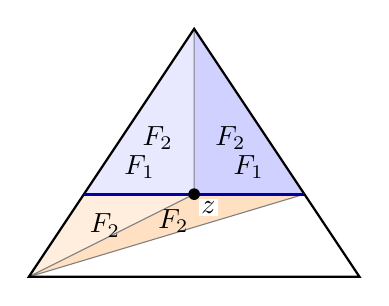
\begin{tikzpicture}[scale=1.05]
 \coordinate (A) at (-2,0);
 \coordinate (B) at (2,0);
 \coordinate (C) at (0,3);
 \coordinate (L) at (-1.3333,1);
 \coordinate (R) at (1.3333,1);
 \coordinate (z) at (0,1);
 \fill[blue!9] (L)--(z)--(C)--cycle;
 \fill[blue!18] (z)--(R)--(C)--cycle;
 \fill[orange!13] (L)--(z)--(A)--cycle;
 \fill[orange!24] (z)--(R)--(A)--cycle;
 \draw[thin,gray] (z)--(A) (A)--(R) (z)--(C);
 \draw[thick] (A)--(B)--(C)--cycle;
 \draw[very thick,blue!65!black] (L)--(R);
 \fill (z) circle (2pt) node[below right=2pt,fill=white,inner sep=1pt] {$z$};
 \node at (-0.44,1.68) {$F_2$};
 \node at (0.44,1.68) {$F_2$};
 \node at (-1.08,0.62) {$F_2$};
 \node at (-0.25,0.67) {$F_2$};
 \node[above=2pt] at (-0.66,1) {$F_1$};
 \node[above=2pt] at (0.66,1) {$F_1$};
\end{tikzpicture}
\caption{The flag count in dimension two. The point $z\in Z_0$ has
two possible incident edges $F_1$ along its one-dimensional carrier.
Each edge has at most two incident triangles $F_2$ inside the original
two-dimensional carrier. The four shaded triangles give the four possible
flags through $z$ in this example. The unshaded triangle has no
one-dimensional-stratum edge through $z$.}
\label{fig:flags}
\end{figure}

Let $\psi:E_n\to\C$ be the invariant cocycle in
Theorem~\ref{thm:sparse}. For an original top simplex $\sigma$, put
\[
 M_\sigma=
 \max_{v_0,\ldots,v_n\in W_\sigma}
 \left|\psi(\delta_{v_0}\wedge\cdots\wedge\delta_{v_n})\right|.
\]
This is finite, even though $\psi$ need not be bounded on all
basis simplices of the infinite vertex set. Every vector in
\eqref{eq:component-average} is a nonnegative convex combination
of vertices in $W_\sigma$. Multilinearity therefore bounds the
evaluation of each surviving term by $M_\sigma$. The preceding
lemma and Proposition~\ref{prop:zero-strata} give
\begin{align}
 \left|\psi\bigl(F^\epsilon(\sigma)\bigr)\right|
 &\leq 2^n M_\sigma
 \int_X\#\bigl(Z_0(x)\cap\sigma\bigr)\,d\mu(x)
 \notag\\
 &\leq 2^n M_\sigma C_\sigma\epsilon
 \longrightarrow 0.\label{eq:small-chain-evaluation}
\end{align}
All constants here are independent of $\epsilon$. Since chains
have finite support, the same convergence holds on every fixed
$c\in C_n(K)$.

\subsection{Equivariant comparison and passage to coinvariants}

It remains to show that the small evaluations just obtained equal
the original cocycle evaluation on every coinvariant cycle.
We do this by constructing a homotopy before taking coinvariants.

\begin{lemma}\label{lem:equivariant-homotopy}
Let $K$ be a simplicial complex with an $H$-action and finite
setwise simplex stabilizers. Let $E_*$ be the augmented exterior
chain complex on a nonempty $H$-set. Any two $H$-equivariant
augmented chain maps $A,B:C_*(K)\to E_*$ that agree in degree $-1$
are $H$-equivariantly chain homotopic.
\end{lemma}

\begin{proof}
The target is acyclic as an augmented complex. Indeed, for any
fixed vertex $v$, the operator $a\mapsto\delta_v\wedge a$ satisfies
\[
 \partial(\delta_v\wedge a)+\delta_v\wedge\partial a=a.
\]
This contraction need not be equivariant. We use it only to choose
finite fillers and then impose equivariance by finite averaging.

Set $h_{-1}=0$. Suppose the homotopy has been constructed below
degree $j$. For an oriented $j$-simplex $e$, the residual
\[
 r(e)=A(e)-B(e)-h_{j-1}(\partial e)
\]
is a cycle, by the chain-map identities and the previously
constructed homotopy. Choose a finite chain $t$ with
$\partial t=r(e)$. Let $S$ be the setwise stabilizer of $e$ and
let $\chi:S\to\{1,-1\}$ be its orientation character, so that
$s e=\chi(s)e$. The residual is equivariant, and hence
$s r(e)=\chi(s)r(e)$. Define
\[
 \overline t=\frac1{|S|}\sum_{s\in S}\chi(s)\,s t.
\]
Then $\partial\overline t=r(e)$ and
$s\overline t=\chi(s)\overline t$. Choose such a filler for one
oriented representative of every simplex orbit, put
$h_j(e)=\overline t$, and extend equivariantly and linearly.
The orientation-character identity makes the extension
well-defined, including when the stabilizer reverses orientation.
This gives $A-B=\partial h+h\partial$ in degree $j$ and completes
the induction.
\end{proof}

\begin{proof}[Proof of Theorem~\ref{thm:sparse}]
The geometric construction applies for every sufficiently large
$n$ depending only on $D$, as fixed by \eqref{eq:strict-volume}.
For nonempty $K$, construct $F^\epsilon$ as above. The stabilizers
are finite by Lemma~\ref{lem:proper}, and $F^\epsilon$ and inclusion
$\iota$ both induce the identity in augmented degree $-1$.
Lemma~\ref{lem:equivariant-homotopy} supplies an equivariant
homotopy
\[
 \iota-F^\epsilon=\partial h+h\partial.
\]

Let $\overline c$ be a cycle of $C_n(K)_H$ and choose a finite
chain lift $c\in C_n(K)$. We do not assume that $c$ is a cycle
before taking coinvariants. Its boundary is a finite sum of
differences $ha-a$. Equivariance of the homotopy makes
$h_{n-1}(\partial c)$ another such sum, which the invariant
functional $\psi$ annihilates. The cocycle identity annihilates
$\partial h_n(c)$. Thus, for every $\epsilon>0$,
\[
 \psi\bigl(\iota(c)\bigr)
 =\psi\bigl(F^\epsilon(c)\bigr).
\]
The right-hand side tends to zero by
\eqref{eq:small-chain-evaluation}, whereas the left-hand side
does not depend on $\epsilon$. Hence it is zero. The evaluation
depends only on the coinvariant class because $\psi$ is invariant.
For empty $K$ there is no nonzero top chain to consider.
\end{proof}

\section{Cycles from an idempotent}
\label{sec:idempotents}

We now return to group rings.  For an idempotent and one infinite-order
conjugacy class, we will construct cycles in every positive even degree.
Their vertices follow steps in one fixed graph of bounded degree. In
sufficiently high dimension, the supporting complexes will therefore
satisfy the hypotheses of Theorem~\ref{thm:sparse}. We first record why
it suffices to perform this construction for finitely generated groups.

The use of cyclic idempotent expressions and reduced centralizers has
its conceptual background in Connes's pairing with projective classes
\cite[Part II, Section 2, Proposition 14]{Connes1985} and Burghelea's
conjugacy-class decomposition \cite[Theorem I]{Burghelea1985}. Our finite
path identities and the detector's normalization are proved directly;
no cyclic-homology identification is assumed.

\begin{lemma}[Subgroup locality]\label{lem:locality}
Let $i:L\hookrightarrow G$ be an inclusion of discrete groups.  Extension
of scalars defines $i_*:K_0(\C L)\to K_0(\C G)$, and for every
$y\in K_0(\C L)$ and $C\in\con(G)$,
\begin{equation}\label{eq:class-aggregation}
 \HS_G(i_*y)(C)
 =\sum_{\substack{B\in\con(L)\\ B\subseteq L\cap C}}
       \HS_L(y)(B).
\end{equation}
Only finitely many terms are nonzero.  Moreover, every
$x\in K_0(\C G)$ is induced from a finitely generated subgroup, which may
be required to contain any prescribed finite subset of $G$.
Consequently, the finite-order-support assertion of
Theorem~\ref{thm:bass} for all finitely generated groups implies that
assertion for all discrete groups.
\end{lemma}

\begin{proof}
We regard free right modules as columns: an idempotent
$e\in M_r(\C L)$ acts on the left, with image $e(\C L)^r$.
Tensoring the split decomposition defined by $e$ with $\C G$ identifies
the extended image with $e(\C G)^r$.  The coefficient sum in an ambient
class $C$ is the sum of its coefficient sums over all $L$-classes contained
in $L\cap C$.  This proves \eqref{eq:class-aggregation} for the image of an
idempotent and then, by subtraction, for every virtual class.  Finiteness
follows from the finite coefficient support of the matrices representing
that class.

Write an arbitrary $x\in K_0(\C G)$ as the difference of the classes of
two finite idempotent matrices.  The group generated by their coefficient
supports and the prescribed finite subset is finitely generated.  The
same matrices are idempotent over its group ring, since that ring embeds
in $\C G$, and their difference induces $x$.  Finally, if an ambient class
consists of infinite-order elements, so does every subgroup class occurring
in \eqref{eq:class-aggregation}: subgroup inclusion preserves the order of
an element.  Vanishing of each subgroup coefficient therefore gives
vanishing of the ambient coefficient.  This uses all the subgroup classes
in the sum, since an ambient conjugacy class can split into several of
them.
\end{proof}

\subsection{A fixed graph and finite path sums}

For the rest of this section, fix a finitely generated group $G$, an
idempotent $e\in M_r(\C G)$, and an infinite-order element $g\in G$.
Write
\[
 e=\sum_{s\in G}A_s s,\qquad A_s\in M_r(\C),\qquad
 S_0=\{s\in G:A_s\ne0\}.
\]
The set $S_0$ is finite.  Idempotence says that
$\sum_{uv=t}A_uA_v=A_t$ for every $t\in G$.  Thus the matrix-valued kernel
\[
 a(h,h')=A_{h^{-1}h'}
\]
is invariant under simultaneous left translation and satisfies
\begin{equation}\label{eq:kernel-idempotence}
 \sum_{k\in G}a(h,k)a(k,h')
 =\sum_{uv=h^{-1}h'}A_uA_v
 =a(h,h').
\end{equation}
All these sums are finite.  In particular, the order of the matrix
factors agrees with the column convention for right modules.

Put
\[
 J=C_G(g),\qquad H=J/\langle g\rangle,\qquad
 Y=\langle g\rangle\backslash G,
 \qquad \bar h=\langle g\rangle h.
\]
Choose a finite symmetric generating set $S\subset G\setminus\{1\}$
containing $S_0\setminus\{1\}$ and its inverses.  Give $Y$ the simple
undirected graph whose edges join $\bar h$ to $\overline{hs}$ for $s\in S$;
loops are omitted and repeated edges identified.  The graph is connected
and has degree at most the fixed integer
\[
 D=\max\{2,|S|\}.
\]
The group $H$ acts by left multiplication.  This is well-defined because
$J$ centralizes $g$, and it preserves right-step edges.  It is free on
vertices: $\overline{ch}=\bar h$ with $c\in J$ implies $ch=g^q h$ for an
integer $q$, and hence $c=g^q$.  Both $H$ and $Y$ are countable.  We keep
this graph and this value of $D$ throughout all subsequent choices of
dimension.

For $k\ge1$, let $Q_k=J\backslash G^k$, with simultaneous left
translation on tuples.  Define the weight of a tuple by
\begin{equation}\label{eq:path-weight}
 w_k(h_0,\ldots,h_{k-1})
 =\tr\bigl(a(h_0,h_1)\cdots
 a(h_{k-2},h_{k-1})a(h_{k-1},gh_0)\bigr),
\end{equation}
where $w_1(h_0)=\tr(a(h_0,gh_0))$.  These weights are $J$-invariant.
They define a finite complex linear combination $v_k$ of elements of
$Q_k$.  Indeed, a nonzero weight has increments
\[
 s_i=h_i^{-1}h_{i+1}\quad(0\le i<k-1),\qquad
 s_{k-1}=h_{k-1}^{-1}gh_0
\]
in $S_0$, with
\[
 s_0\cdots s_{k-1}=h_0^{-1}gh_0.
\]
An increment list determines the tuple from $h_0$.  Any two choices of
$h_0$ with this conjugate differ by left multiplication in $J$, so the
list determines at most one element of $Q_k$.  Hence $v_k$ has at most
$|S_0|^k$ nonzero coefficients.  For a $J$-invariant function $p$ on
$G^k$, write $v_k(p)$ for the finite weighted sum of its values.  These
weights need not be real or positive.

\begin{lemma}[Path identities]\label{lem:path-identities}
For the path sums associated to $e$ and $g$, the twisted cyclic shift
\[
 T(h_0,\ldots,h_{k-1})=(h_1,\ldots,h_{k-1},gh_0)
\]
preserves $v_k$.  For $k\ge2$, deletion of any entry induces a map
$d_i:Q_k\to Q_{k-1}$ satisfying
\[
 (d_i)_*v_k=v_{k-1}\qquad(0\le i<k).
\]
Every $v_k$ has the same total weight
\begin{equation}\label{eq:trace-coefficient}
 \lambda:=v_k(1)
 =\sum_{s\in[g]_G}\tr(A_s)
 =\HS_G\bigl([e(\C G)^r]\bigr)([g]_G).
\end{equation}
\end{lemma}

\begin{proof}
The shift $T$ is a $J$-equivariant bijection, with inverse
\[
 (h_0,\ldots,h_{k-1})\longmapsto
 (g^{-1}h_{k-1},h_0,\ldots,h_{k-2}).
\]
For $k=1$, the shift is the identity on $Q_1$, since $g\in J$.
For $k\ge2$, the shifted weight has the factors of
\eqref{eq:path-weight} in cyclic order, since
$a(gh_0,gh_1)=a(h_0,h_1)$.  Cyclicity of the matrix trace proves
$T_*v_k=v_k$.

For deletion, fix a representative of the shorter tuple.  Each orbit in
its fibre has a unique representative with exactly those retained
entries, because simultaneous left translation acts freely on any
nonempty tuple.  Thus the fibre sum is over the missing entry in $G$,
without a stabilizer factor.  Internal deletions follow from
\eqref{eq:kernel-idempotence}, as does deletion of the last entry using
\[
 \sum_u a(h_{k-2},u)a(u,gh_0)=a(h_{k-2},gh_0).
\]
For the first deletion, fix $(h_1,\ldots,h_{k-1})$ and put
$B=a(h_1,h_2)\cdots a(h_{k-2},h_{k-1})$, with $B=I_r$ when $k=2$.
Then
\begin{align*}
 &\sum_{h_0}\tr\bigl(a(h_0,h_1)B a(h_{k-1},gh_0)\bigr)\\
 &\qquad=\sum_{h_0}\tr\bigl(Ba(h_{k-1},gh_0)a(gh_0,gh_1)\bigr)\\
 &\qquad=\tr\bigl(Ba(h_{k-1},gh_1)\bigr).
\end{align*}
Here the first equality uses trace cyclicity and left invariance; the
second uses \eqref{eq:kernel-idempotence} with the substitution $u=gh_0$.
This also proves the assertion for $k=2$.  The kernel has finite row and
column support, so every fibre sum used in these computations is finite.

The deletion identities show that all total weights equal $v_1(1)$.
Finally,
\[
 J\backslash G\longrightarrow[g]_G,\qquad Jh\longmapsto h^{-1}gh
\]
is a bijection: equality of the conjugates is equivalent to
$h'h^{-1}\in J$.  Therefore
$v_1(1)=\sum_{s\in[g]_G}\tr(A_s)$, which is precisely the indicated
Hattori--Stallings coefficient.
\end{proof}

\subsection{Even-dimensional cycles}

The path identities now turn the finite sums into cycles.  We use the
exterior complex $E_*$ on the graph $Y$.
For $k\ge1$, define
\[
 \pi_k:\C^{(Q_k)}\longrightarrow(E_{k-1})_H,\qquad
 [h_0,\ldots,h_{k-1}]\longmapsto
 [\delta_{\bar h_0}\wedge\cdots\wedge\delta_{\bar h_{k-1}}].
\]
The map is well-defined because changing a tuple by an element of $J$
changes its projected vertices by a simultaneous $H$-translation.
Set $b_k=\pi_k(v_k)$, and, for $n=2m\ge2$, set
\[
 z_n=b_{n+1}\in(E_n)_H.
\]

\begin{proposition}\label{prop:path-cycle}
For every positive even integer $n$, the chain $z_n$ is a cycle.
Moreover, either its defining sum has no nonzero distinct-vertex terms,
so $z_n=0$, or it is the image of a cycle in $C_n(K)_H$ for an
$H$-invariant simplicial complex $K$ generated by $n$-simplices, with
finitely many simplex orbits, whose top vertex sets span connected
subgraphs of $Y$.  The graph and its degree bound $D$ are independent
of $n$.
\end{proposition}

\begin{proof}
Since $\overline{gh_0}=\bar h_0$, the twisted shift projects to the cyclic
permutation of the $k$ wedge factors.  Hence
\[
 \pi_kT=(-1)^{k-1}\pi_k.
\]
Together with $T_*v_k=v_k$, this shows that $b_k=0$ whenever $k$ is even.
The deletion identities give
\[
 \partial b_k=\sum_{i=0}^{k-1}(-1)^i b_{k-1}\qquad(k\ge2).
\]
For even $n$, it follows that $\partial z_n=b_n=0$.

A tuple with repeated projected vertices contributes zero to the wedge.
For every remaining tuple with nonzero weight, consecutive projected
vertices are joined by edges from the fixed step set $S$.  Their path
visits all its $n+1$ vertices, so the subgraph spanned by those vertices
is connected.  Let $K$ be generated by these vertex sets and their
$H$-translates.  Finite support of $v_{n+1}$ gives finitely many orbits
of top simplices and of their faces.

The same finite expression for $z_n$ defines a chain in $C_n(K)_H$.
To see that its boundary is zero there, decompose $E_j$ in every degree
as the direct sum of the span of the oriented simplices belonging to
$K$ and the span of all other oriented simplices.  Both summands are
$H$-invariant, including their orientation signs.  Thus
\[
 E_j=C_j(K)\oplus W_j,
 \qquad
 (E_j)_H=C_j(K)_H\oplus(W_j)_H.
\]
In particular the inclusion remains injective after taking
coinvariants.  The boundary of the chain in $C_n(K)_H$ maps to
$\partial z_n=0$, so it is zero already in $C_{n-1}(K)_H$.
\end{proof}

We have obtained the required sparse cycles in arbitrarily large even
degrees.  The underlying path sums all have total weight $\lambda$, the trace
coefficient in \eqref{eq:trace-coefficient}. The next section constructs
a cocycle whose value on $z_{2m}$ recovers a nonzero scalar multiple of
that coefficient.

\section{A Pfaffian cocycle detecting the trace coefficient}
\label{sec:detector}

Retain the finitely generated group $G$, idempotent, infinite-order element
$g$, and notation $J,H,Y,v_k,\lambda,z_{2m}$ of
Section~\ref{sec:idempotents}.  We construct an $H$-invariant cocycle whose
value on $z_{2m}$ is $2^{-m}\lambda$.  The construction first records the
relative powers of $g$ between two lifts of vertices of $Y$.  An alternating
Pfaffian expression will then remove the dependence on those lifts.

\subsection{Relative exponents between lifts}

\begin{lemma}\label{lem:beta}
There is a $J$-invariant function $\beta:G\times G\to\R$ such that
\begin{equation}\label{eq:beta-properties}
 \beta(h',h)=-\beta(h,h'),\qquad
 \beta(g^r h,g^s h')=\beta(h,h')+s-r
 \quad(r,s\in\Z).
\end{equation}
\end{lemma}

\begin{proof}
The diagonal $H$-action on the set of ordered pairs $Y\times Y$ is free,
because its action on the first coordinate is free.  This also applies to
diagonal pairs $(y,y)$.  For each orbit choose a representative $(y_o,y'_o)$
and lifts $(l_o,l'_o)\in G^2$.  For $(h,h')\in G^2$, there is a unique
$\bar c\in H$ carrying the appropriate representative to the projected
pair.  Choose a lift $c\in J$ and write
\[
 h=g^r c l_o,\qquad h'=g^s c l'_o.
\]
For fixed $c$, the integers $r,s$ are unique because $g$ has infinite order.
Replacing $c$ by $g^t c$ replaces them by $r-t,s-t$.  Thus
$B(h,h')=s-r$ is well defined.  Commutation with $g$ shows that $B$ is
$J$-invariant, and independently changing the two lifts gives
\[
 B(g^a h,g^b h')=B(h,h')+b-a.
\]
The antisymmetrization
\[
 \beta(h,h')=\frac{B(h,h')-B(h',h)}2
\]
has all the required properties.
\end{proof}

The function $\beta$ itself need not descend to $Y\times Y$.  In fact,
\eqref{eq:beta-properties} gives $\beta(h,g^k h)=k$ even though these two
lifts project to the same vertex.  Nor is there a difficulty if an element
$\bar c\in H$ exchanges two distinct projected vertices.  If a lift
$c\in J$ satisfies
$c h_0=g^a h_1$ and $c h_1=g^b h_0$, its invariance merely requires
\[
 2\beta(h_0,h_1)=b-a,
\]
which is precisely what antisymmetrization gives.  Real values are useful
here: for $G=\langle t\rangle$ and $g=t^2$, the value
$\beta(1,t)=1/2$ is forced.

\subsection{The cyclic Pfaffian identity}

In degree two, a lift-independent expression is
\[
 c(y_0,y_1,y_2)
 =\beta(h_1,h_2)-\beta(h_0,h_2)+\beta(h_0,h_1),
 \qquad \bar h_i=y_i.
\]
Changing $h_i$ to $g^{r_i}h_i$ adds
$(r_2-r_1)-(r_2-r_0)+(r_1-r_0)=0$, so $c$ depends only on the
projected vertices. In higher even degrees we replace $\beta$ by a
Pfaffian and take the same alternating deletion sum. The Pfaffian
still depends on the lifts; its deletion sum will define the cocycle.
We first compute the weighted Pfaffian sum, then prove the descent
and cocycle properties of its deletion sum.

For a list $\mathbf h=(h_0,\ldots,h_{2m-1})$ with $m\ge1$, let
\[
 p_m(\mathbf h)=\operatorname{Pf}
       \bigl(\beta(h_i,h_j)\bigr)_{0\le i,j<2m},
 \qquad p_0=1.
\]
We use the convention that $p_m(\mathbf h)$ is the coefficient of
$\varepsilon_0\wedge\cdots\wedge\varepsilon_{2m-1}$ in $b^m/m!$, where
$\varepsilon_i$ are the coordinate one-forms on the space of list positions
and
\[
 b=\sum_{i<j}\beta(h_i,h_j)\,
              \varepsilon_i\wedge\varepsilon_j.
\]
In particular, $p_1(h_0,h_1)=\beta(h_0,h_1)$, and $p_m$ is alternating in
its entries and $J$-invariant.  The finite weighted sums
\[
 q_m=v_{2m}(p_m)\quad(m\ge1),\qquad q_0=\lambda
\]
are therefore defined.  No boundedness of $p_m$ on all lists is needed.

\begin{lemma}\label{lem:pfaffian-recurrence}
For every $m\ge1$, one has $q_m=\tfrac12q_{m-1}$ and hence
$q_m=2^{-m}\lambda$.
\end{lemma}

\begin{proof}
An ordinary cyclic rotation of a list of length $2m$ changes its Pfaffian
by the sign $(-1)^{2m-1}=-1$.  In the twisted rotation
\[
 T\mathbf h=(h_1,\ldots,h_{2m-1},g h_0),
\]
replacing the last entry $h_0$ by $g h_0$ adds $1$ to every matrix entry in
the last column above the diagonal.  Expansion along that column gives
\begin{equation}\label{eq:pfaffian-rotation}
 \begin{split}
 p_m(T\mathbf h)
   ={}&-p_m(\mathbf h)\\
     &+\sum_{i=1}^{2m-1}(-1)^{i+1}
       p_{m-1}(h_1,\ldots,\widehat{h_i},\ldots,h_{2m-1}).
 \end{split}
\end{equation}
Indeed the last-column cofactor in position $i$, with positions numbered
$1,\ldots,2m$, has sign $(-1)^{i+1}$; each Pfaffian matching uses exactly
one entry from that column.

For $m\ge2$, each minor on the second line omits $h_0$ and $h_i$ from the
original list.  Applying the deletion identity in
Lemma~\ref{lem:path-identities} twice shows that its weighted sum under
$v_{2m}$ is $q_{m-1}$.  For $m=1$, the minor is $p_0=1$, whose weighted sum
is the total weight $v_2(1)=\lambda=q_0$.  Thus this endpoint uses no vector
$v_0$.  The invariance of $v_{2m}$ under $T$ and
$\sum_{i=1}^{2m-1}(-1)^{i+1}=1$ now turn
\eqref{eq:pfaffian-rotation} into
\[
 q_m=-q_m+q_{m-1}.
\]
The claimed formulas follow.
\end{proof}

\subsection{Descent to an exterior cocycle}

The preceding calculation detects the coefficient on lists of lifts.
We next descend it to the exterior complex on $Y$, where the sparse-chain
theorem applies.

\begin{proposition}\label{prop:detector}
For every integer $m\ge1$, the formula
\begin{equation}\label{eq:detector-formula}
 \psi_m(y_0,\ldots,y_{2m})
   =\sum_{i=0}^{2m}(-1)^i
       p_m(h_0,\ldots,\widehat{h_i},\ldots,h_{2m}),
\end{equation}
where $h_i\in G$ is any lift of $y_i\in Y$, defines an $H$-invariant
linear functional $\psi_m:E_{2m}\to\C$ satisfying
\[
 \psi_m\partial=0,\qquad
 \psi_m(z_{2m})=2^{-m}\lambda.
\]
Here evaluation on the coinvariant chain $z_{2m}$ is defined by
$H$-invariance.
\end{proposition}

\begin{proof}
On the $2m+1$ list positions put
\[
 u=\sum_{i=0}^{2m}\varepsilon_i,
 \qquad
 b=\sum_{0\le i<j\le2m}\beta(h_i,h_j)\,
                         \varepsilon_i\wedge\varepsilon_j.
\]
The right side of \eqref{eq:detector-formula} is the coefficient of the
ordered top form in $u\wedge b^m/m!$.  Moving the factor
$\varepsilon_i$ past its $i$ preceding positions gives exactly the sign
$(-1)^i$ in that formula.

Changing the lifts to $g^{r_i}h_i$ replaces $\beta(h_i,h_j)$ by
$\beta(h_i,h_j)+r_j-r_i$.  Thus it replaces $b$ by
$b+u\wedge v$, with $v=\sum_i r_i\varepsilon_i$.  Every correction term
in $u\wedge(b+u\wedge v)^m$ contains two factors $u$ and vanishes.
This proves independence of the lifts.

The expression is alternating in the lifted list.  After lift independence
has been established, it is therefore alternating in the projected
vertices as well.  In particular, if two projected vertices coincide,
choose equal lifts for them to see that the expression vanishes.  It
consequently defines a linear functional on
$E_{2m}=\bigwedge^{2m+1}\C^{(Y)}$.
For $\bar c\in H$, choose $c\in J$ and use $c h_i$ as the lifts of the
translated vertices.  The $J$-invariance of $\beta$ proves the
$H$-invariance of $\psi_m$.

To check the cocycle identity, choose lifts simultaneously for a list of
$2m+2$ vertices.  On every face, \eqref{eq:detector-formula} is the
alternating deletion coboundary of $p_m$ on these same lifts.  A second
deletion cancels each twice-omitted list in its two possible orders.
Hence $\psi_m\partial=0$.

Finally, $z_{2m}$ is the exterior projection of $v_{2m+1}$.
Each one-deletion term in \eqref{eq:detector-formula} has weighted sum
$v_{2m}(p_m)=q_m$, by Lemma~\ref{lem:path-identities}.  Since
$\sum_{i=0}^{2m}(-1)^i=1$, their signed sum gives
\[
 \psi_m(z_{2m})=q_m=2^{-m}\lambda,
\]
using Lemma~\ref{lem:pfaffian-recurrence}.  Repeated projected vertices
already have zero exterior image and zero value under $\psi_m$, so they
require no separate restriction in this evaluation.
\end{proof}

\section{Completion of the trace theorem}
\label{sec:completion}

We now combine the geometric vanishing with the detector. The order of
the choices matters: the graph is fixed by the idempotent before its
cycle dimension is chosen.

\begin{proof}[Proof of Theorem~\ref{thm:bass}]
First let $G$ be finitely generated, let $e\in M_q(\C G)$ be an
idempotent, and fix an infinite-order $g\in G$. Construct the graph on
$Y=\langle g\rangle\backslash G$ and the free action of
$H=C_G(g)/\langle g\rangle$ as in Section~\ref{sec:idempotents}.
Let $D\geq2$ be a degree bound for this fixed graph, and choose an even
integer $n=2m\geq n_0(D)$ with $m\geq1$.

Proposition~\ref{prop:path-cycle} gives the cycle $z_n$, and
Proposition~\ref{prop:detector} gives an $H$-invariant cocycle
$\psi_m:E_n\to\C$ with
\[
 \psi_m(z_n)=2^{-m}\lambda,
 \qquad
 \lambda=\HS_G([e(\C G)^q])([g]_G).
\]
If no nonzero simplices occur, $z_n=0$ and this identity already gives
$\lambda=0$. Otherwise Proposition~\ref{prop:path-cycle} realizes $z_n$
as a cycle in $C_n(K)_H$ for an $H$-invariant complex $K$ satisfying all
hypotheses of Theorem~\ref{thm:sparse}. That theorem gives
$\psi_m(z_n)=0$, with the same conclusion. Every finitely generated
projective right $\C G$-module is represented by an idempotent, and every element of
$K_0(\C G)$ is a difference of two such classes. Additivity proves the
assertion for all finitely generated groups.

For an arbitrary discrete group $G$, choose idempotents representing
$x\in K_0(\C G)$ and let $G_0\leq G$ be generated by $g$ and all group
elements occurring in their entries. Then $G_0$ is finitely generated
and $x=i_*x_0$ for some $x_0\in K_0(\C G_0)$, where $i:G_0\hookrightarrow G$.
Lemma~\ref{lem:locality} expresses $\HS_G(x)([g]_G)$ as the sum of the
coefficients $\HS_{G_0}(x_0)(C)$ over those $G_0$-conjugacy classes
$C\subseteq G_0\cap[g]_G$. Only finitely many terms are nonzero, and
every element in every such class has infinite order. Each term
vanishes by the finitely generated case.
\end{proof}

\subsection{The integral trace}

For the integral group ring, the same idempotent formula defines
\[
 \HS_{\Z G}:K_0(\Z G)\longrightarrow
 \Z G/[\Z G,\Z G]\cong\bigoplus_{C\in\con(G)}\Z C,
\]
where commutators are now taken with their additive span. The integral
Bass trace conjecture asks for support only at the identity class.

\begin{corollary}\label{cor:integral}
For every discrete group $G$, the Hattori--Stallings trace of every
class in $K_0(\Z G)$ is supported on $[1]_G$.
\end{corollary}

\begin{proof}
If $P$ is a finitely generated projective right $\Z G$-module, the same
idempotent matrix over $\C G$ represents $P\otimes_{\Z G}\C G$.
Consequently its trace coefficients are the images under
$\Z\hookrightarrow\C$ of those of $P$. Theorem~\ref{thm:bass} and this
coefficientwise injection give vanishing at all infinite-order elements.
No injectivity assertion about the map between the two $K_0$ groups is
required.

For finite-order elements we use Linnell's restriction
\cite[Lemma 4.1]{Linnell1983}, in the form stated and reproved by
Berrick and Hesselholt \cite[Theorem A]{BH2015}: if the integral trace of a finitely
generated projective module is nonzero at $h$, there is an integer
$a\geq1$ such that $h$ is conjugate to $h^{s^a}$ for every integer
$s\geq1$. Their convention also uses right modules.
If $h$ has finite order $t>1$, take $s=t$.
Then $h^{t^a}=1$, so the restriction would make $h$ conjugate to $1$,
a contradiction. Thus every nonidentity finite-order coefficient also
vanishes. Taking differences of projective classes finishes the proof.
\end{proof}

\subsection{Homotopy idempotents and Lefschetz numbers}

The integral support statement also has fixed-point consequences.
A self-map $f$ is a \emph{homotopy idempotent} if $f\circ f\simeq f$.
Such a map on a connected finite CW complex $X$ admits maps
$u:X\to Y$ and $v:Y\to X$ with
\[
 v\circ u\simeq f,\qquad u\circ v\simeq\id_Y
\]
\cite[Section 3]{BCM2006}. The second identity says that $Y$ is
\emph{finitely dominated} by $X$. For a pointed homotopy idempotent
with $f_\#=\id_G$, where $G=\pi_1(X)$, the induced maps $u_\#$ and
$v_\#$ identify $\pi_1(Y)$ with $G$. The universal-cover chains of $Y$
are chain homotopy equivalent to a finite complex $P_*$ of finitely
generated projective $\Z G$-modules. The sum
$\sum_i(-1)^i[P_i]\in K_0(\Z G)$ is its projective Euler class. The
Hattori--Stallings trace of this class records the fixed-point class indices of $f$:
it is the Reidemeister trace, with conjugacy classes inverted when
passing from the left-module convention of \cite[Lemma 4.1]{BCM2006}
to ours. The augmentation trace and the identity coefficient of this projective
class give the ordinary and $L^2$-Lefschetz numbers, respectively
\cite[Lemmas 8.1--8.2]{BCM2006}. Berrick, Chatterji and Mislin use these
relations to deduce the following consequences of the integral support
statement and its numerical trace consequence.

\begin{corollary}[Berrick--Chatterji--Mislin consequences]
\label{cor:homotopy-idempotents}
Let $M$ be a connected closed smooth oriented manifold.
\begin{enumerate}[label=\textup{(\roman*)}]
 \item If $\dim M>2$ and $f:M\to M$ satisfies $f\circ f\simeq f$
 by free homotopy, then some self-map freely homotopic to $f$ has
 exactly one fixed point.
 \item Choose $x_0\in M$ and put $G=\pi_1(M,x_0)$. If
 $f:(M,x_0)\to(M,x_0)$ satisfies $f\circ f\simeq_* f$ by based
 homotopy and $f_\#=\id_G$, then
 \[
  L(f)=L^{(2)}(\widetilde f).
 \]
 Here $\widetilde f$ is the lift to the universal cover fixing a chosen
 point above $x_0$; it is $G$-equivariant. The left side is the ordinary
 Lefschetz number, and the right side is the alternating sum of von
 Neumann traces on the induced $L^2$-homology maps, as in
 \cite[Definition 7.1]{BCM2006}.
\end{enumerate}
\end{corollary}

\begin{proof}
For $x\in K_0(\Z G)$ write $h_C(x)=\HS_{\Z G}(x)(C)$. The
augmentation trace $\epsilon$ is the sum of these coefficients, while
the Kaplansky trace $\kappa$ is the identity coefficient. The sum is
finite, and Corollary~\ref{cor:integral} gives
\[
 \epsilon(x)=\sum_{C\in\con(G)}h_C(x)=h_{[1]_G}(x)=\kappa(x).
\]
This is the weak Bass conjecture for every group. The cited paper uses
projective left modules, whereas we use right modules. The anti-involution
$g\mapsto g^{-1}$, together with transpose on idempotent matrices,
transports between these conventions and relabels the coefficient at
$[g]_G$ by $[g^{-1}]_G$. It preserves identity support and both
$\epsilon$ and $\kappa$. Thus Corollary~\ref{cor:integral} gives the
classical Bass conjecture in the cited convention, and the displayed
equality gives weak Bass there. The forward implications of
\cite[Theorem 1]{BCM2006} and \cite[Theorem 2]{BCM2006} now give
\textup{(i)} and \textup{(ii)}, respectively.
\end{proof}

\section{Torsion-free groups: trace rank and idempotents}
\label{sec:torsion-free}

For a torsion-free group, the support theorem leaves only the identity
conjugacy class. We first identify its coefficient with augmentation
rank, and then use the two possible scalar ranks to determine scalar
idempotents.

\begin{proof}[Proof of Corollary~\ref{cor:torsion-free}\textup{(i)}]
Let $e\in M_q(\C G)$ be idempotent and put
$x=[e(\C G)^q]\in K_0(\C G)$. Since $G$ is torsion-free,
Theorem~\ref{thm:bass} says that $\HS_G(x)$ is supported on $[1]_G$.
Therefore
\begin{align}
 \tau_{G,q}(e)
 &=\HS_G(x)([1]_G)\notag\\
 &=\sum_{C\in\con(G)}\HS_G(x)(C)\notag\\
 &=\epsilon_G\!\left(\sum_{i=1}^q e_{ii}\right)
 =\tr\bigl(\epsilon_{G,q}(e)\bigr)
 =\operatorname{rank}_{\C}\bigl(\epsilon_{G,q}(e)\bigr).
 \label{eq:torsion-free-rank}
\end{align}
The class sum is finite because the entries of $e$ have finite group
support. The last
equality holds because $\epsilon_{G,q}(e)$ is an idempotent complex
matrix: its image-kernel decomposition makes its trace equal to its
rank. Taking differences of projective classes gives
$\tau_{G,*}=\operatorname{rk}_{\epsilon}$. This map has range exactly
$\Z$, since its values are integers and $[\C G]$ has value $1$.
\end{proof}

For matrices the conclusion is numerical. For example,
$\operatorname{diag}(1,0)\in M_2(\C G)$ is an idempotent other than zero
and the identity, with augmentation rank one. The scalar case is special
because its augmentation rank can only be zero or one.

\begin{proof}[Proof of Corollary~\ref{cor:torsion-free}\textup{(ii)}]
First take $R=\C$ and let $e\in\C G$ be idempotent. Equation
\eqref{eq:torsion-free-rank} with $q=1$ gives
\[
 \tau_G(e)=\epsilon_G(e)\in\{0,1\}.
\]
We use the standard faithful-trace argument, as in
\cite[Theorem 2.1 and Remark 2.2]{BV1998}, spelling out a similarity
to a projection. Embed $\C G$ by left convolution in the group von
Neumann algebra $\mathcal N(G)$, the commutant of the right regular
representation on $\ell^2(G)$. Its canonical normalized trace is
\[
 \tau_G(T)=\langle T\delta_1,\delta_1\rangle .
\]
Its faithfulness can be seen directly: if
$T\geq0$ and $\tau_G(T)=0$, then $T^{1/2}\delta_1=0$. Since $T^{1/2}$
commutes with right translations and their translates of $\delta_1$
span a dense subspace, $T^{1/2}=0$, hence $T=0$.

Set
\[
 a=e^*e+(1-e)^*(1-e).
\]
For every $\xi\in\ell^2(G)$,
\[
 \langle a\xi,\xi\rangle
 =\|e\xi\|^2+\|(1-e)\xi\|^2
 \geq \tfrac12\|\xi\|^2.
\]
Thus $a$ is positive and invertible in $\mathcal N(G)$, and a direct
multiplication gives $ae=e^*a$. With $s=a^{1/2}$, the element
$p=ses^{-1}$ satisfies $p^2=p$ and
$p^*=s^{-1}e^*s=ses^{-1}=p$. Hence $p$ is a projection, and
traciality gives $\tau_G(p)=\tau_G(e)$. If this value is zero,
faithfulness applied to $p=p^*p$ gives $p=0$. If it is one,
faithfulness applied to $1-p$ gives $p=1$. Similarity then gives
$e=0$ or $e=1$.

Now let $R$ be any commutative unital domain of characteristic zero
and write an idempotent $f\in RG$ as
$f=\sum_{g\in S}r_g g$ with $S$ finite. Put
\[
 R_0=\Z[r_g:g\in S]\subseteq R,\qquad F=\operatorname{Frac}(R_0).
\]
The field $F$ is finitely generated over $\mathbb Q$, and therefore
embeds in $\C$. Indeed, send a finite transcendence basis of
$F/\mathbb Q$ to an algebraically independent tuple of complex
numbers; the resulting embedding of the rational function field
extends across the finite algebraic extension $F$ because $\C$ is
algebraically closed. The coefficientwise maps
$R_0G\hookrightarrow RG$ and $R_0G\hookrightarrow\C G$ are injective.
Thus $f^2=f$ already holds in $R_0G$, and its image in $\C G$ is an
idempotent. The complex case makes that image $0$ or $1$, and
injectivity gives the same conclusion for $f$. Only the finitely
generated coefficient field $F$ was embedded; no embedding of all
of $R$ into $\C$ is required.
\end{proof}

\begin{remark}[Algebraic and completed trace ranges]
Continue to assume that $G$ is torsion-free. Let
$j:\C G\hookrightarrow C_r^*(G)$ be the inclusion into the reduced
group $C^*$-algebra, and let
\[
 j_*:K_0(\C G)\longrightarrow K_0^{\mathrm{top}}(C_r^*(G))
\]
be the comparison map to topological $K$-theory. Write
$\tau_*^{\mathrm{top}}:K_0^{\mathrm{top}}(C_r^*(G))\to\R$ for the
canonical trace pairing. It agrees with $\tau_{G,*}$ on this image:
the same positive similarity used above, applied in a matrix algebra
over $C_r^*(G)$, produces a projection representing the image of a
matrix idempotent, and traciality preserves its trace. Consequently
\[
 \tau_*^{\mathrm{top}}\!\left(j_*K_0(\C G)\right)=\Z.
\]
This is the integer range on the algebraic image, not a statement
about every class of $K_0^{\mathrm{top}}(C_r^*(G))$. In particular,
the argument does not presume that the algebraic augmentation extends
to the reduced completion. The stronger completed idempotent question
is the Kadison--Kaplansky conjecture; see \cite[Section 1]{OW2023}.

The coefficient reduction above uses characteristic zero. An idempotent
$e\notin\{0,1\}$ would give nonzero zero divisors through $e(1-e)=0$,
so the zero-divisor conjecture would imply the idempotent conjecture.
The reverse implication is not established here.
\end{remark}

\bibliographystyle{plain}
\bibliography{references}
\end{document}
